\chapter{Quantum droplet of hetero-nuclear Bose mixture}
\label{Chap_droplet}

% epigraph (done 2021-9-30 09:06:25)
\setlength{\unitlength}{1pt}
\setlength{\epigraphwidth}{10cm}
\epigraph{Law of physicists I: \\ Without experimentalists, theorists tend to drift. \cite{Lee:1992ui}}{--- T.D. Lee\\ \textit{History of the weak interactions (1987)}}

% 历史在这里讲

% Overview and structure of theory part of this chapter (done 2021-10-7 20:49:40)
This chapter discusses the heteronuclear droplets formed by the Bose-Einstein condensate mixture of Na and Rb. We first re-analyze the droplet, however, with a finite volume instead of homogeneous density distribution. This is to compare with experiments since an actual quantum droplet we build in the experiment always has a specific size due to a limited atomic number. We make a rough estimation by analyzing the energy scales of each term. Then, continuing with the analytical solution in Sec. \ref{sec:droplet_ana}, we implement the variational calculation. We use a simple Gaussian trial function to help understand how different energy scales compete in the finite-size droplets. Its specific size mainly requires introducing a kinetic energy term (i.e. quantum pressure). In order to better understand the droplet sample, we simulate it with extended Gross–Pitaevskii equation (eGPE). In this part, we give the derivation of the extended GPE especially for the two-species BEC sample near zero MF energy region. We put the code of GPELAB \cite{ANTOINE20142969} and samples of the simulation results in the Appendix \ref{chap:eGPELAB} with more details.

% Overview and structure of experiment part of this chapter (done 2021-10-7 22:54:47)
In Sec. \ref{sec:droplet_experiment}, we experimentally study Na-Rb droplet and measure the phase diagram of liquid-gas phase transition, which is the central part of our experimental research. The experimental method is simple and straightforward. We directly let the sample do Time-of-Flight and observe the non-expansion signal. This method avoids the complexity of the optical-levitation method however need more effort to eliminate the inhomogeneity of the magnetic field. In order to cooperate with this scheme, we upgrade our system on both control of magnetic field and imaging method, referring to Sec. \ref{sec:image} and Sec. \ref{sec:fastcoil} for details. Later, in Sec. \ref{sec:LHY_gas}, we study the gaseous LHY sample. This research aims to explore the behaviour of a gaseous sample under the dominance of LHY energy instead of MF energy. This research is a supplement to the study of LHY gas by measuring the trap frequency \cite{skov2020}. After understanding the droplet formation process, we realize that the previous process of preparing droplets is far from adiabatic, which resulted in significant limitations on the sample life and the number of atoms. So we improve the preparation scheme to achieve a droplet sample with more numbers as shown in Sec. \ref{sec:mode_match}. Finally, Sec. \ref{sec:droplet_molecule} shows our efforts on using droplets to form the Feshbach molecules. Although the conversion efficiency has no improvement, we have greatly reduced the temperature of the molecules and provide a promising path for the future production of degenerate Feshbach molecules.


\section{Quantum droplet with finite size}
\label{sec:finite_size}

% overall of this section (done 2021-10-8 09:20:57)
In Sec. \ref{sec:droplet_ana}, we calculate the quantum liquid analytically, showing the mean-field and LHY energy expressions. Then we obtain the equilibrium density of the system. This calculation ignores the system's quantum pressure (kinetic energy), which means it is only proper for homogeneous bulk samples. However, in our experiments, due to the limitation of the atomic number, we currently cannot obtain a sample with a large enough number allowing us to ignore its edge. Thus, in this section, we first analyse the quantum pressure caused by the finite volume then show its influence on the quantum liquid droplet. 

% introducing energy expression (done 2021-10-14 23:14:55)
The total energy of the system consists of three parts; in addition to the interaction energy (Mean-field energy and LHY correction), there is also the quantum pressure due to the finite size of the sample. This can also be explained by the uncertainty principle since the finite size can be viewed as a size limitation and will introduce a finite momentum (energy). The total energy expression of this finite-size droplet sample is
\begin{equation}
\begin{split}
E_{\text{total}}&=E_{\text{kin}}+E_{\text{MF}}+E_{\text{LHY}}\\
E_{\text{kin}}&=N \frac{\hbar ^2}{2m}\int \left| \nabla \phi (\pmb{r})\right| ^2 \, dr^3\\
E_{\text{MF}}&=\frac{g}{2}N^2\int \left| \phi (\pmb{r})\right| ^4 \, dr^3,\quad g=\frac{2\pi  \hbar ^2a_S}{m/2}
\end{split}
\end{equation}
where $N$ is particle number, $m$ is its mass, $g$ is the interaction strength which is proportional to scattering length $a_S$. Note that here we write down the formula with only single species, however later we need to extend it to double species case, which is just summation along two species for all $N$ and $g_{ij}$. The LHY correction expression needs an infinite integration which is will be explained later.

% explain three terms (done 2021-10-22 11:46:21)
Locally, MF energy is proportional to $n^2$, and LHY correction is proportional to $n^{5/2}$. The kinetic energy (quantum pressure) is proportional to the square of the derivation of the wave function. For a homogeneous bulk sample, just as we mentioned in Chap. \ref{Chap:theory}, the quantum pressure term is zero. However, considering a finite size sample, the rapid decreasing of the wave function on the boundary (the density inside is limited and the outside is the vacuum) introduces additional kinetic energy. This kinetic energy tends to reduce the variation rate of the wave function (density) on the boundary. So it tends to inflate the sample. This term does not exist in a classic system but only in a quantum system which is the same as the LHY term. 

% surface tension and core pressure (done 2021-10-22 11:47)
Another phenomenon called surface tension can be explained by MF energy on the boundary. At the boundary, density is lower than at the core part, and the positive energy of LHY is much smaller than the attraction energy of MF. So the attraction force is dominated by MF energy and offer surface tension similar to the classical liquid. From another perspective, MF energy is a zero-order approximation, both existing in classical and quantum systems. This surface tension will cause the pressure at the core to be higher than the homogeneous sample. In the finite droplet case, because the environment is with zero pressure, thus the core of the sample will have a pressure higher than zero. This can be offered by the LHY term, as we mentioned in Chap. \ref{Chap:theory}, the LHY term increase faster than the MF term with increasing density. So, the LHY repulsion overcomes the MF attraction at the core and support the sample without collapsing.

% droplet density distribution (done 2021-10-22 12:24:37)
\begin{figure}[htb]
\begin{center}
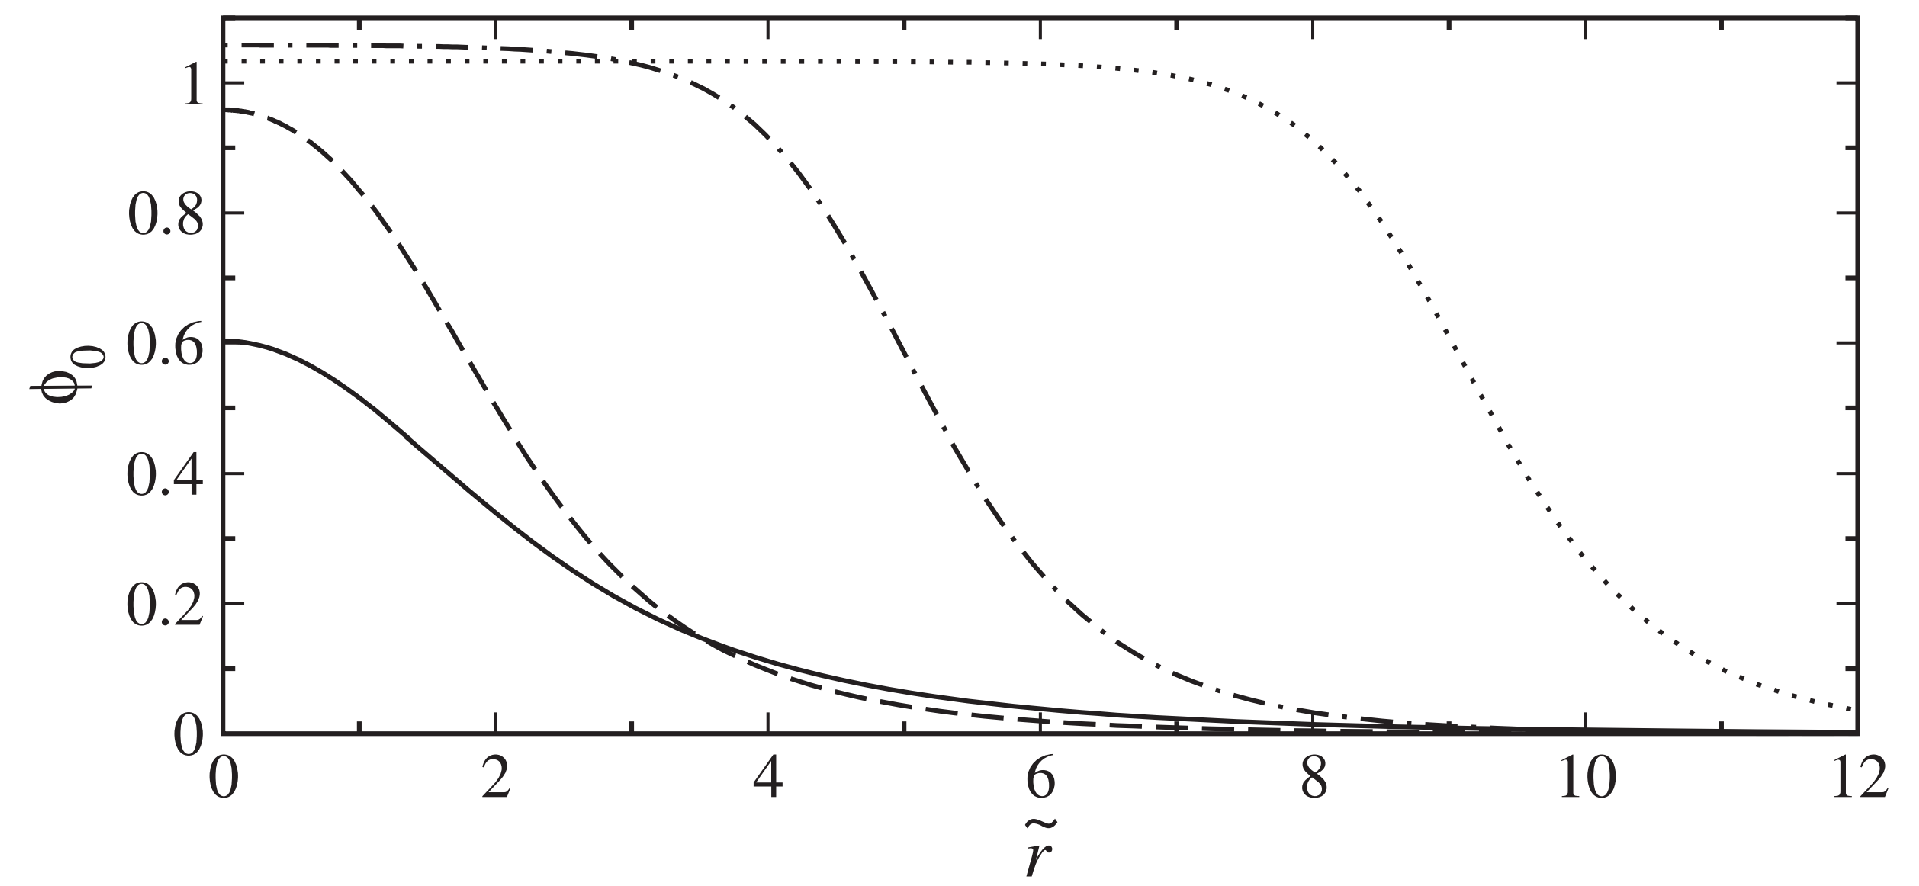
\includegraphics[width = 0.8\linewidth]{droplet_density_dis.pdf}
\end{center}
\caption[Droplet density distribution and edge effect]{Figure shows the density distribution of a finite-size droplet. The edge size is of about one $\hat{r}$ which provides the surface tension. Figure from \cite{petrov2015}.}
\label{droplet_density_dis}
\end{figure}

% quantum droplet with trap (done 2021-10-22 12:11:21)
In addition to the quantum droplet of free space, we also discuss the sample of in trap. For the in-trap sample, we need to add an additional energy term of the trap. So, the total energy is made of four parts now. For a sample with finite size, trap energy and quantum pressure behaves opposite. Small size introduces higher quantum pressure but reduces trap energy and vice versa. This is similar for MF and LHY energy, where MF energy is negative; however, LHY energy is positive. For samples with specific sizes, these two-term compete with each other. Analyzing such a sample with two groups of energies competing with each other is not straightforward. Therefore, the calculation of the variational method we introduced in Sec. \ref{sec:var_cal} can help us understand better. This part is explained carefully in sec. For more detailed calculations, please refer to \cite{Liu2020}.

\section{Variational calculation}
\label{sec:var_cal}

% overall of this section (done 2021-10-14 23:28:26)
In this section, we introduce the variational calculation of droplets. Variational calculations can help us better understand the energy competition in the system. From the analysis in the previous section, we can read that whatever the quantum pressure or the interaction energy in a quantum droplet of finite volume,  they all depend on the system's wave function distribution. Thus, a pure analytical calculation lacks information and can not reveal how these different energies compete with each other.

% why we use variational method instead of directly using GPE simulation (done 2021-10-14 23:47:19)
A more accurate method is the finite element method, which treats the entire wave function as a function of space coordinates. Then it uses a variational method to adjust the value of the wave function at each spatial position, reducing the overall system's energy, thereby providing a more accurate solution. However, the calculation of the three-dimensional system consumes vast computing resources, which is incapable of ordinary personal computers. In order to understand the behaviour of the system, we need an intermediate model to help us establish the relationship between various causes and effects. After this step, the subsequent GPE simulation will be more straightforward.

% section structure (done 2021-10-29 20:56:48)
This section first reviews the variational calculation of single species BEC and defines the so-called release energy. We explain how release energy reflects the interaction and the measurement of the second-order correlation function. At the same time, this also gives an experimental measurement method, i.e. the direct TOF method. Then we show the introduction of the Gaussian variational method in the double-species system. Although it is a very rough approximation, the calculation should be pretty effective for the case with a relatively small atomic number and the droplet sample far away from the top-flat density distribution at the centre. This will be verified in subsequent calculations. We imitate the dimensionless parameters of the single-species BEC and introduce two dimensionless parameters to characterize the double-species BEC in the trap. Thereby it is convenient to describe the system and compare it with different species combinations.

% more details (done 2021-10-29 21:03:11)
We calculate two items by the variational method: 1. LHY gas in a harmonic trap and the released energy when expansion in free-space. 2. Droplet with magnetic field gradient and how the critical number is shifting. We start from a single BEC in a harmonic trap and review the variational method with Gaussian Ansatz. Noted that, we get the $\chi $= - 0.67 there is a collapse point, which offers no solution. Then, we plot the release energy curve. The release energy is just the sum of kinetic energy in the trap plus the interaction energy. For the Double BEC near-zero MF energy, the behaviour of the sample is very similar to a single BEC, as the $\lambda_+$ branch requires minimum density, leaving only the $\lambda_-$ branch. So, assuming that Na and Rb share the same wave function, we can use the result from the single BEC part. By choosing the correct characteristic value, we can make a comparison for experimental data.

% GPE vs. variational method (done 2021-10-29 21:05:50)
We also use the eGPE to calculate the release energy in Sec. \ref{sec:eGPE}, due to Gaussian Ansatz does not fit for large atomic number cases. We find a great overlap between our experiment and the eGPE simulation. In comparing the MF and LHY cases, we can say that we measured the LHY energy for the zero-MF with a shift from 0.75$\hbar \omega $ to about 1.3 $\hbar\omega$. This relatively large shift is definite beyond MF theory. The eGPE simulation cannot give out physics explanation. However, the variational method can. So, we plot all kinds of energy as a function of the variational parameter $w$. This plot can explain several questions: 1. How do these different energies compete? What is the meaning of the meta-stable state of a droplet? 2. What parameter do we need to characterize the LHY term? Moreover, how large is this term compared to the MF term and others? 3. what will happen if the initial state does not match the droplet state? Will the expansion over the local maximum and miss the droplet formation?

% more(done 2021-10-29 21:06:08)
Finally, we add one more variational parameter to the Gaussian Ansatz to explain the shift of critical numbers when the magnetic field gradient exists. The main idea is that Na and Rb wavefunction will surfer a tiny centre shifting $\delta $, which decrease the absolute value of Mean-Field energy between Na and Rb. Because the $E_{\text{MF$\_$Rb}-\text{Na}}$ is the product of their density. So the overlap will change dramatically. However, The rest part of MF and LHY energy will keep. So, this gradient will decrease the binding term when we are in the droplet region, which shifts the critical number above.

\subsection{Single species BEC in harmonic trap}

% Hamiltonian and energy (done 2021-10-16 06:58:29)
We first recall the textbook result of the variational solution about a single BEC in harmonic trap. Here, we introduce the Gaussian ansatz as an approximation. Considering N Bosons in a harmonic trap with trap frequency of $\omega _0$, its ground state energy is made of 
\begin{equation}
\begin{split}
E_{\text{kin}}&=N \frac{\hbar ^2}{2m}\int \left| \nabla \phi (\pmb{r})\right| ^2 \, dr^3\\
E_{\text{trap}}&=N\int \left| \phi (\pmb{r})\right| ^2V_{\text{trap}}(\pmb{r})dr^3,\text{   }V_{\text{trap}}(\pmb{r})=\frac{1}{2}m \omega _0^2\pmb{r}^2\\
E_{\text{MF}}&=\frac{g}{2}N^2\int \left| \phi (\pmb{r})\right| ^4 \, dr^3,\quad g=\frac{2\pi  \hbar ^2a_S}{m/2}
\end{split}
\end{equation}
where we for now ignore the LHY correction. For convenience we define the harmonic length $a_{\text{ho}}=\sqrt{\frac{\hbar }{m \omega _0}}$.

% Gaussian ansatz and variational energy (done 2021-10-16 07:03:10)
Now, we use variational method to calculate the wave-function in trap. the Gaussian ansatz is 
\begin{equation}
\phi (\pmb{r})=\frac{1}{\pi^{3/4}\left(w^3a_{\text{ho}}^3\right){}^{1/2}}e^{-\frac{\pmb{r}^2}{2w^2a_{\text{ho}}^2}}
\end{equation}
where the $w$ is the variational parameter. Then, we have
\begin{equation}
\begin{split}
E_{\text{kin}}&=N \frac{\hbar^2}{2m}\int \left|\nabla\phi(\pmb{r})\right|^2 dr^3=N\hbar\omega_0\frac{3}{4w^2}\\
E_{\text{trap}}&=N\int\left|\phi(\pmb{r})\right| ^2 V_{\text{trap}}(\pmb{r})dr^3 = N\hbar\omega_0\left(\frac{3}{4} w^2\right)\\
E_{\text{MF}}&=\frac{g}{2}N^2\int\left|\phi(\pmb{r})\right|^4dr^3=N \hbar\omega_0\left(\frac{1}{\sqrt{2\pi}}\frac{a_SN}{a_{\text{ho}}}\frac{1}{w^3}\right)
\end{split}
\end{equation}
i.e. total energy 
\begin{equation}
E_{\text{tot}}(w)=N\hbar\omega_0\left(\frac{3}{4}\frac{1}{w^2}+\frac{3}{4}w^2+\frac{1}{\sqrt{2\pi}}\frac{a_SN}{a_{\text{ho}}}\frac{1}{w^3}\right)
\end{equation}

% minimize energy to get ground state (done 2021-10-16 07:03:00)
Then we minimize the $E_{\text{tot} }$ with the constrain of $\int\phi\phi^*dr^3=N$
\begin{equation}
E_{\text{tot}}(w)-\mu N=N \hbar  \omega _0\left(\frac{3}{4}\frac{1}{w^2}+\frac{3}{4}w^2+\frac{1}{\sqrt{2\pi }}\frac{a_SN}{a_{\text{ho}}}\frac{1}{w^3}\right)-\mu  N
\end{equation}
To get the $w$ of ground state, we take the derivative of $E_{\text{tot}}$
\begin{equation}
{\partial _w\left(\frac{3}{4}\frac{1}{w^2}+\frac{3}{4}w^2+\frac{1}{\sqrt{2\pi }}\frac{\chi }{w^3}\right)}=-\frac{3}{2 w^3}+\frac{3 w}{2}-\frac{3 \chi }{\sqrt{2 \pi } w^4}
\end{equation}
where we use $\chi $ represent the dimensionless quantity $\frac{a_SN}{a_{\text{ho}}}$.

\begin{itemize}[noitemsep,topsep=0pt]
    \item If tuning $g=0$, i.e. the non-interacting case, we get back to the single particle picture. The wave-function is a Gaussian with size of harmonic length, i.e. $w=1$
    \item With increasing $\chi $, we have larger size (larger $w$), and finally, when reach $\chi >>1$ limit, we turn to the Thomas-Fermi limit.
    \item For $\chi <0$, we have attractive Bose gas, with collapse point at $\chi =-0.671$ \cite{}
\end{itemize}

\subsection{Double BEC in harmonic trap with near zero-MF interaction}

% Hamiltonian and energy
Now we turn to our double species case, i.e. $N_{\text{Rb}}$ Rb and $N_{\text{Na}}$ Na in a harmonic trap with trap frequency of $\omega_{\text{Rb}}$ and $\omega _{\text{Na}}$, we have ground state energy of
\begin{equation}
\begin{split}
E_{\text{kin}}&=N_{\text{Na}}\frac{\hbar^2}{2m_{\text{Na}}}\int \left| \nabla \phi _{\text{Na}}(\pmb{r})\right|^2dr^3+N_{\text{Rb}}\frac{\hbar ^2}{2m_{\text{Rb}}}\int\left|\nabla\phi_{\text{Rb}}(\pmb{r})\right|^2dr^3\\
E_{\text{trap}}&=N_{\text{Na}}\int\left|\phi_{\text{Na}}(\pmb{r})\right|^2V_{\text{trap}-\text{Na}}(\pmb{r})dr^3+N_{\text{Rb}}\int\left|\phi _{\text{Rb}}(\pmb{r})\right|^2V_{\text{trap}-\text{Rb}}(\pmb{r})dr^3\\
E_{\text{MF}}&=\frac{g_{\text{Na}}}{2}N_{\text{Na}}^2\int\left|\phi_{\text{Na}}(\pmb{r})\right|^4dr^3+\frac{g_{\text{Rb}}}{2}N_{\text{Rb}}^2\int\left|\phi_{\text{Rb}}(\pmb{r})\right|^4dr^3\\
&\qquad\qquad\qquad\qquad+g_{\text{Rb},\text{Na}}N_{\text{Na}}N_{\text{Rb}}\int\left|\phi_{\text{Rb}}(\pmb{r})\right|^2\left|\phi_{\text{Na}}(\pmb{r})\right|^2dr^3\\
E_{\text{LHY}}&=\int\frac{256\sqrt{\pi}\hbar^2}{15}\left(m_{\text{Na}}^{-2/5}a_{\text{Na}}\left|\phi_{\text{Na}}(\pmb{r})\right|^2+m_{\text{Rb}}^{-2/5}a_{\text{Rb}}\left|\phi_{\text{Rb}}(\pmb{r})\right|^2\right)^{5/2}dr^3
\end{split}
\end{equation}
where
\begin{equation}
\begin{split}
&V_{\text{trap}-\text{Rb}}(\pmb{r})=\frac{1}{2}m_{\text{Rb}}\omega _{\text{Rb}}^2\pmb{r}^2,V_{\text{trap}-\text{Na}}(\pmb{r})=\frac{1}{2}m_{\text{Na}} \omega _{\text{Na}}^2\pmb{r}^2\\
g_{\text{Rb}}&=\frac{2\pi\hbar^2a_{\text{Rb}}}{\left.m_{\text{Rb}}\right/2},\text{}g_{\text{Na}}=\frac{2\pi\hbar^2a_{\text{Na}}}{\left.m_{\text{Na}}\right/2},\text{     }g_{\text{Rb},\text{Na}}=\frac{2\pi  \hbar ^2a_{\text{Rb},\text{Na}}}{m_{\text{Rb}}m_{\text{Na}}/\left(m_{\text{Rb}}+m_{\text{Na}}\right)}\\
\end{split}    
\end{equation}
As we are dealing with the case of $E_{\text{MF}}\to 0$, we can make several approximation:
\begin{itemize}[noitemsep,topsep=0pt]
    \item Two BECs share the same wave-function $\phi (\pmb{r})$
    \item Gaussian Ansatz
\end{itemize}
With the first approximation, we can rewrite the Hamiltonian as
\begin{equation*}
\begin{split}
E_{\text{kin}}&=\left(\frac{N_{\text{Na}}}{m_{\text{Na}}} +\frac{N_{\text{Rb}}}{m_{\text{Rb}}}\right)\frac{\hbar ^2}{2}\int \left| \nabla \phi (\pmb{r})\right|^2 dr^3=\frac{N}{m} \frac{\hbar ^2}{2}\int \left| \nabla \phi (\pmb{r})\right| ^2 \, dr^3\\
E_{\text{trap}}&=\frac{1}{2}\left(m_{\text{Rb}} \omega _{\text{Rb}}^2N_{\text{Rb}}+m_{\text{Na}} \omega _{\text{Na}}^2N_{\text{Na}}\right)\int \left|\phi (\pmb{r})\right| ^2\pmb{r}^2dr^3=\frac{1}{2}m \omega ^2N\int \left| \phi (\pmb{r})\right| ^2\pmb{r}^2dr^3\\
E_{\text{MF}}&=\frac{g_{\text{Na}}N_{\text{Na}}^2+g_{\text{Rb}}N_{\text{Rb}}^2+2g_{\text{Rb},\text{Na}}N_{\text{Na}}N_{\text{Rb}}}{2}\int \left| \phi(\pmb{r})\right| ^4 \, dr^3=\frac{g}{2}N^2\int \left| \phi (\pmb{r})\right| ^4 \, dr^3\\
E_{\text{LHY}}&=\frac{8\left(m_{\text{Na}}^{3/5}g_{\text{Na}}N_{\text{Na}}+m_{\text{Rb}}^{3/5}g_{\text{Rb}}N_{\text{Rb}}\right)^{5/2}}{15\pi ^2\hbar ^3}\int\left| \phi (\pmb{r})\right| ^5dr^3=\frac{8m^{3/2}\Gamma ^{5/2}N^{5/2}}{15\pi ^2\hbar ^3}\int \left| \phi (\pmb{r})\right| ^5 dr^3
\end{split}
\end{equation*}
Now, we recover to the single component case, with new mass, number, trap frequency and interaction strength following \pmb{ the negative branch} as shown in \cite{petrov2015}
\begin{equation}
E_{\text{MF}-}=\lambda _-n_-^2, \quad\text{with}\quad \lambda _-=\frac{\text{$\delta$g}\sqrt{g_{\text{Rb}}g_{\text{Na}}}}{\left(g_{\text{Na}}+g_{\text{Rb}}\right)}\quad\text{and}\quad n_-=\frac{n_{\text{Rb}}\sqrt{g_{\text{Na}}}+n_{\text{Na}}\sqrt{g_{\text{Rb}}}}{\sqrt{g_{\text{Na}}+g_{\text{Rb}}}}
\end{equation}
Thus, we can define the new number and interaction strength as
\begin{equation}
\begin{split}
N&=N_-=\frac{N_{\text{Rb}}\sqrt{g_{\text{Na}}}+N_{\text{Na}}\sqrt{g_{\text{Rb}}}}{\sqrt{g_{\text{Na}}+g_{\text{Rb}}}}\\
g&=\frac{4\pi  \hbar ^2a_S}{m}=2\lambda _-=\frac{2\text{$\delta $g}\sqrt{g_{\text{Rb}}g_{\text{Na}}}}{\left(g_{\text{Na}}+g_{\text{Rb}}\right)},\text{  }\text{$\delta $g}=g_{\text{Rb},\text{Na}}+\sqrt{g_{\text{Rb}}g_{\text{Na}}}
\end{split}
\end{equation}
Then, we have
\begin{equation}
\begin{split}
m&=\frac{N m_{\text{Na}}m_{\text{Rb}}}{N_{\text{Na}}m_{\text{Rb}}+N_{\text{Rb}}m_{\text{Na}}}\\
\omega&=\sqrt{\frac{\left(N_{\text{Na}}m_{\text{Rb}}+N_{\text{Rb}}m_{\text{Na}}\right)\left(m_{\text{Rb}}\omega_{\text{Rb}}^2N_{\text{Rb}}+m_{\text{Na}}\omega_{\text{Na}}^2N_{\text{Na}}\right)}{N^2m_{\text{Na}}m_{\text{Rb}}}}\\
\Gamma&=\frac{m_{\text{Na}}^{3/5}g_{\text{Na}}N_{\text{Na}}+m_{\text{Rb}}^{3/5}g_{\text{Rb}}N_{\text{Rb}}}{m^{3/5}N}=\frac{4\pi  \hbar ^2A}{m}
\end{split}
\end{equation}
For convenience we define the harmonic length
\begin{equation}
a_{\text{ho}}=\sqrt{\frac{\hbar }{m \omega }}=\sqrt{\hbar \sqrt{\frac{N_{\text{Na}}m_{\text{Rb}}+N_{\text{Rb}}m_{\text{Na}}}{\left(m_{\text{Rb}}
\omega _{\text{Rb}}^2N_{\text{Rb}}+m_{\text{Na}} \omega _{\text{Na}}^2N_{\text{Na}}\right)m_{\text{Na}}m_{\text{Rb}}}}}
\end{equation}
With Gaussian Ansatz
\begin{equation}
\phi (\pmb{r})=\frac{1}{\pi ^{3/4}\left(w^3a_{\text{ho}}^3\right){}^{1/2}}e^{-\frac{\pmb{r}^2}{2w^2a_{\text{ho}}^2}}
\end{equation}
We get the similar formula as the single BEC near zero-MF point, and its total energy is
\begin{equation}
E_{\text{tot}}(w)=N\hbar\omega\left(\frac{3}{4}\frac{1}{w^2}+\frac{3}{4}w^2+\frac{1}{\sqrt{2\pi}}\chi\frac{1}{w^3}+\frac{512}{75 \pi ^{7/4}}\sqrt{\frac{2}{5}}\xi\frac{1}{ w^{9/2}}\right)
\end{equation}
where
\begin{equation}
\chi =\frac{a_SN}{a_{\text{ho}}}, \xi =\left(\frac{A}{a_{\text{ho}}}\right){}^{5/2}N^{3/2}
\end{equation}

%%%%%%%%%%%%%%%%%%%%%%%%%%%%%%%%%%%%
% finish to here 2021-10-15 20:56:29


Released energy is

\begin{equation}E_{\text{release}}=\frac{\left(\frac{3}{2}m_{\text{Rb}}N_{\text{Rb}}v_{\text{Rb}}^2+\frac{3}{2}m_{\text{Na}}N_{\text{Na}}v_{\text{Na}}^2\right)}{N}\end{equation}

\begin{equation}
\begin{split}
\frac{E_{\text{release}}}{\hbar\omega_{\text{ho}}}&=\frac{\left(\frac{3}{2}m_{\text{Rb}}N_{\text{Rb}}v_{\text{Rb}}^2+\frac{3}{2}m_{\text{Na}}N_{\text{Na}}v_{\text{Na}}^2\right)}{N}\frac{1}{\hbar\sqrt{\frac{\left(N_{\text{Na}}m_{\text{Rb}}+N_{\text{Rb}}m_{\text{Na}}\right)\left(m_{\text{Rb}}\omega _{\text{Rb}}^2N_{\text{Rb}}+m_{\text{Na}} \omega _{\text{Na}}^2N_{\text{Na}}\right)}{N^2m_{\text{Na}}m_{\text{Rb}}}}}\\
&=\frac{\left(m_{\text{Rb}}N_{\text{Rb}}v_{\text{Rb}}^2+m_{\text{Na}}N_{\text{Na}}v_{\text{Na}}^2\right)}{2\hbar}\frac{3\sqrt{m_{\text{Na}}m_{\text{Rb}}}}{\sqrt{\left(N_{\text{Na}}m_{\text{Rb}}+N_{\text{Rb}}m_{\text{Na}}\right)\left(m_{\text{Rb}}\omega_{\text{Rb}}^2N_{\text{Rb}}+m_{\text{Na}}\omega _{\text{Na}}^2N_{\text{Na}}\right)}}
\end{split}
\end{equation}

about the $\chi $

\begin{equation}\chi =\frac{a_SN}{a_{\text{ho}}}=\frac{g \frac{m_{\text{Na}}m_{\text{Rb}}}{N_{\text{Na}}m_{\text{Rb}}+N_{\text{Rb}}m_{\text{Na}}}}{4\pi  \hbar
^2}\frac{\left(\frac{N_{\text{Rb}}\sqrt{g_{\text{Na}}}+N_{\text{Na}}\sqrt{g_{\text{Rb}}}}{\sqrt{g_{\text{Na}}+g_{\text{Rb}}}}\right){}^2}{\sqrt{\hbar
\sqrt{\frac{N_{\text{Na}}m_{\text{Rb}}+N_{\text{Rb}}m_{\text{Na}}}{\left(m_{\text{Rb}} \omega _{\text{Rb}}^2N_{\text{Rb}}+m_{\text{Na}} \omega _{\text{Na}}^2N_{\text{Na}}\right)m_{\text{Na}}m_{\text{Rb}}}}}}\end{equation}

about the $\xi $

\begin{equation}\xi =\left(\frac{A}{a_{\text{ho}}}\right){}^{5/2}N^{3/2}=\left(\frac{\left(\frac{ m_{\text{Na}}m_{\text{Rb}}}{N_{\text{Na}}m_{\text{Rb}}+N_{\text{Rb}}m_{\text{Na}}}\right){}^{2/5}}{4\pi
 \hbar ^2}\frac{m_{\text{Na}}^{3/5}g_{\text{Na}}N_{\text{Na}}+m_{\text{Rb}}^{3/5}g_{\text{Rb}}N_{\text{Rb}}}{\sqrt{\hbar \sqrt{\frac{N_{\text{Na}}m_{\text{Rb}}+N_{\text{Rb}}m_{\text{Na}}}{\left(m_{\text{Rb}}
\omega _{\text{Rb}}^2N_{\text{Rb}}+m_{\text{Na}} \omega _{\text{Na}}^2N_{\text{Na}}\right)m_{\text{Na}}m_{\text{Rb}}}}}}\right){}^{5/2}\end{equation}

\subsection{How magnetic field gradient affect droplet}

When we put $N_{\text{Rb}}$ Rb and $N_{\text{Na}}$ Na in free space, with magnetic gradient $\nabla $B, we take the center-of-mass as original point.
Consider gradient force
\begin{equation}
F=N_{\text{Rb}}\mu _{\text{Rb}}\nabla B+N_{\text{Na}}\mu _{\text{Na}}\nabla B
\end{equation}
The acceleration of whole sample is
\begin{equation}
\mathcal{A}_{\text{center of mass}}=F/m=\frac{N_{\text{Rb}}\mu _{\text{Rb}}+N_{\text{Na}}\mu _{\text{Na}}}{N_{\text{Rb}}m_{\text{Rb}}+N_{\text{Na}}m_{\text{Na}}}\nabla B
\end{equation}
So, in the coordinate of center of mass, we have Na and Rb with acceleration on different direction
\begin{equation}
\mathcal{A}_{\text{Rb}}=\frac{\mu _{\text{Rb}}\nabla B}{m_{\text{Rb}}}-\frac{N_{\text{Rb}}\mu _{\text{Rb}}\nabla B+N_{\text{Na}}\mu _{\text{Na}}\nabla
B}{N_{\text{Rb}}m_{\text{Rb}}+N_{\text{Na}}m_{\text{Na}}}
\end{equation}
\begin{equation}
\mathcal{A}_{\text{Na}}=\frac{\mu _{\text{Na}}\nabla B}{m_{\text{Na}}}-\frac{N_{\text{Rb}}\mu _{\text{Rb}}\nabla B+N_{\text{Na}}\mu _{\text{Na}}\nabla
B}{N_{\text{Rb}}m_{\text{Rb}}+N_{\text{Na}}m_{\text{Na}}}
\end{equation}
and their relationship is
\begin{equation}
m_{\text{Rb}}\mathcal{A}_{\text{Rb}}N_{\text{Rb}}=-m_{\text{Na}}\mathcal{A}_{\text{Na}}N_{\text{Na}}
\end{equation}
Now, we can take gradient as an external field and the formula of the energy coming from this gradient is
\begin{equation}
E_{\text{gradient}}=N_{\text{Na}}m_{\text{Na}}\mathcal{A}_{\text{Na}}\int \left| \phi _{\text{Na}}(\pmb{r})\right|^2dr^3+N_{\text{Rb}}m_{\text{Rb}}\mathcal{A}_{\text{Rb}}\int\left|\phi _{\text{Rb}}(\pmb{r})\right|^2dr^3
\end{equation}
Other terms of energy as following
\begin{equation}
\begin{split}
E_{\text{kin}}&=N_{\text{Na}}\frac{\hbar^2}{2m_{\text{Na}}}\int\left|\nabla\phi_{\text{Na}}(\pmb{r})\right|^2dr^3+N_{\text{Rb}}\frac{\hbar^2}{2m_{\text{Rb}}}\int\left|\nabla\phi_{\text{Rb}}(\pmb{r})\right|^2dr^3\\
E_{\text{trap}}&=N_{\text{Na}}\int\left|\phi_{\text{Na}}(\pmb{r})\right|^2V_{\text{trap}-\text{Na}}(\pmb{r})dr^3+N_{\text{Rb}}\int\left|\phi_{\text{Rb}}(\pmb{r})\right|^2V_{\text{trap}-\text{Rb}}(\pmb{r})dr^3\\
E_{\text{MF}}&=\frac{g_{\text{Na}}}{2}N_{\text{Na}}^2\int\left|\phi _{\text{Na}}(\pmb{r})\right|^4dr^3+\frac{g_{\text{Rb}}}{2}N_{\text{Rb}}^2\int\left|\phi_{\text{Rb}}(\pmb{r})\right|^4dr^3\\
&\qquad\qquad+g_{\text{Rb},\text{Na}}N_{\text{Na}}N_{\text{Rb}}\int\left|\phi_{\text{Rb}}(\pmb{r})\right|^2\left|\phi_{\text{Na}}(\pmb{r})\right|^2dr^3\\
E_{\text{LHY}}&=\int\frac{256\sqrt{\pi}\hbar^2}{15}\left(m_{\text{Na}}^{-2/5}a_{\text{Na}}\left|\phi_{\text{Na}}(\pmb{r})\right|^2+m_{\text{Rb}}^{-2/5}a_{\text{Rb}}\left|\phi_{\text{Rb}}(\pmb{r})\right|^2\right)^{5/2}dr^3
\end{split}
\end{equation}
where
\begin{equation}
\begin{split}
V_{\text{trap}-\text{Rb}}(\pmb{r})&=\frac{1}{2}m_{\text{Rb}}\omega _{\text{Rb}}^2\pmb{r}^2\\
V_{\text{trap}-\text{Na}}(\pmb{r})&=\frac{1}{2}m_{\text{Na}} \omega _{\text{Na}}^2\pmb{r}^2\\
g_{\text{Rb}}&=\frac{2\pi\hbar^2a_{\text{Rb}}}{\left.m_{\text{Rb}}\right/2}\\
g_{\text{Na}}&=\frac{2\pi\hbar^2a_{\text{Na}}}{\left.m_{\text{Na}}\right/2}\\
g_{\text{Rb},\text{Na}}&=\frac{2\pi\hbar^2a_{\text{Rb},\text{Na}}}{m_{\text{Rb}}m_{\text{Na}}/\left(m_{\text{Rb}}+m_{\text{Na}}\right)}
\end{split}
\end{equation}
Gaussian Ansatz with center shifts
\begin{equation}
\begin{split}
\phi _{\text{Na}}(x,y,z)=\frac{1}{\pi ^{3/4}\left(w^3a_{\text{ho}}^3\right){}^{1/2}}e^{-\frac{x^2+\left(y-\frac{m_{\text{Rb}}N_{\text{Rb}}\delta
_y}{m_{\text{Rb}}N_{\text{Rb}}+m_{\text{Na}}N_{\text{Na}}}\right){}^2+z^2}{2w^2a_{\text{ho}}^2}}\\
\phi _{\text{Rb}}(x,y,z)=\frac{1}{\pi ^{3/4}\left(w^3a_{\text{ho}}^3\right){}^{1/2}}e^{-\frac{x^2+\left(y+\frac{m_{\text{Na}}N_{\text{Na}}\delta
_y}{m_{\text{Rb}}N_{\text{Rb}}+m_{\text{Na}}N_{\text{Na}}}\right){}^2+z^2}{2w^2a_{\text{ho}}^2}}
\end{split}
\end{equation}
Then, we have 
\begin{equation}
\begin{split}
E_{\text{kin}}&=N_{\text{Na}}\frac{\hbar^2}{2m_{\text{Na}}}\int\left|\nabla\phi_{\text{Na}}(\pmb{r})\right|^2dr^3+N_{\text{Rb}}\frac{\hbar^2}{2m_{\text{Rb}}}\int\left|\nabla\phi_{\text{Rb}}(\pmb{r})\right|^2dr^3\\
E_{\text{trap}}&=\frac{1}{2}\left(m_{\text{Rb}}\omega_{\text{Rb}}^2N_{\text{Rb}}+m_{\text{Na}}\omega_{\text{Na}}^2N_{\text{Na}}\right)\int\left|\phi(\pmb{r})\right|^2\pmb{r}^2dr^3=\frac{1}{2}m\omega^2N\int\left|\phi(\pmb{r})\right|^2\pmb{r}^2dr^3\\
E_{\text{MF}}&=\frac{g_{\text{Na}}N_{\text{Na}}^2+g_{\text{Rb}}N_{\text{Rb}}^2+2g_{\text{Rb},\text{Na}}N_{\text{Na}}N_{\text{Rb}}}{2}\int\left|\phi(\pmb{r})\right|^4dr^3=\frac{g}{2}N^2\int\left|\phi(\pmb{r})\right|^4dr^3\\
E_{\text{LHY}}&=\frac{8}{15\pi^2\hbar^3}\left(m_{\text{Na}}^{3/5}g_{\text{Na}}N_{\text{Na}}+m_{\text{Rb}}^{3/5}g_{\text{Rb}}N_{\text{Rb}}\right)^{5/2}\int\left|\phi(\pmb{r})\right|^5dr^3\\
&=\frac{8}{15\pi^2\hbar^3}m^{3/2}\Gamma^{5/2}N^{5/2}\int\left|\phi (r)\right|^5dr^3
\end{split}
\end{equation}
Put the center shift Gaussian into it, we have
\begin{equation}
\begin{split}
E_{\text{tot}}[w]=&N\hbar\omega\left(\left(-\mu_{\text{eff}}\nabla B\right)\delta +\frac{3}{4}\frac{1}{w^2}+\frac{3}{4}w^2+\frac{1}{\sqrt{2\pi}}\frac{a_SN}{a_{\text{ho}}}\frac{1}{w^3}\left(\lambda e^{-\delta^2}\right)\right.\\
&\left.\qquad\qquad\qquad+\frac{512}{75\pi^{7/4}}\sqrt{\frac{2}{5}}\left(\frac{A}{a_{\text{ho}}}\right){}^{5/2}N^{3/2}\frac{1}{w^{9/2}}\right)
\end{split}
\end{equation}
When, $\delta $ is a small value, we have $e^{-\delta ^2}=1-\delta ^2$, thus we have
\begin{equation}
\begin{split}
E_{\text{tot}}[w]&=N\hbar\omega\left[\left(\frac{3}{4}\frac{1}{w^2}+\frac{3}{4}w^2+\frac{1}{\sqrt{2\pi}}\chi\frac{1}{w^3}+\frac{512}{75\pi^{7/4}}\sqrt{\frac{2}{5}}\xi\frac{1}{w^{9/2}}\right)\right.\\\
&\qquad\qquad\qquad\left.+\lambda\delta^2-\left(\mu_{\text{eff}}\nabla B\right)\delta\right]
\end{split}
\end{equation}
where
\begin{equation}
\begin{split}
\chi&=\frac{a_SN}{a_{\text{ho}}}\\
\xi&=\left(\frac{A}{a_{\text{ho}}}\right){}^{5/2}N^{3/2}
\end{split}
\end{equation}

\section{extended GPE solution}
\label{sec:eGPE}

% overall of this section (done 2021-10-15 21:06:03)
Although the variational method used in the previous section provides a general physical image, the method will get meaningless results when the system deviates from the reasonable parameter interval because we use a rough Gauss ansatz. So we need more accurate numerical calculations to compare with experimental data. Since quantum depletion takes only a tiny portion of our system, it is reasonable to use the local density approximation to calculate the wave function of the condensate part. Therefore, we only need to add LHY correction to the MF shift as a high-level correction, then use this extended GPE to calculate the system to get the condensate wave function of the system.

% section structure and adopt Minardi approximation (done 2021-10-17 11:16:11)
In this section, let us first revisit the calculation of MF and LHY correction of the double BEC system. Then we first derive the single species GPE. Then imitating this process, the derivation of the extended GPE of double-species is provided. When calculating the LHY correction, if we adopt the method of infinite integration, the amount of calculation will increase. So we imitated \cite{Minardi2019} and adopted an approximation with an error of less than 15\%. The rationality of this approximation essentially stems from the symmetry of exchanging two species. If two species have the same mass, such as two spin states of the same atomic species, the approximation gets back to the analytical solution as shown in \cite{petrov2015}.

% Hamiltonian (done 2021-10-17 11:23:15)
Hamiltonian for BEC with two components is
\begin{equation}
\begin{split}
H_{\text{tot}}=\sum_k\epsilon_{1,k}\hat{a}_{1,k}^\dagger\hat{a}_{1,k}+&\frac{g_{11}}{2V}\sum_{\left\{k_i\right\}}\hat{a}_{1,k_1}^\dagger\hat{a}_{1,k_2}^\dagger\hat{a}_{1,k_3}\hat{a}_{1,k_4}+\sum_k\epsilon_{2,k}\hat{a}_{2,k}^\dagger\hat{a}_{2,k}\\
&+\frac{g_{22}}{2V}\sum_{\left\{k_i\right\}}\hat{a}_{2,k_1}^\dagger\hat{a}_{2,k_2}^\dagger\hat{a}_{2,k_3}\hat{a}_{2,k_4}+\frac{g_{12}}{V}\sum_{\left\{k_i\right\}}\hat{a}_{2,k_1}^\dagger\hat{a}_{1,k_2}^\dagger\hat{a}_{1,k_3}\hat{a}_{2,k_4}
\end{split}
\end{equation}
where $k_1+k_2=k_3+k_4$, satisfy momentum conservation. $g_{\text{ii}}$ represent intra-interaction strength, and $g_{12}$ for inter-interaction. $\hat{a}_{i,k}^\dagger(\hat{a}_{i,k})$ denote the ladder operator for $i^{\text{th}}$ component, i.e. 
\begin{equation}
\hat{a}_{i,0}=\sqrt{N_i}
\end{equation}

% ground state energy (done 2021-10-17 12:14:10)
As calculated in Chap. \ref{Chap:theory}, ground state energy is
\begin{equation}
\begin{split}
E_{\text{GS}}=&\frac{g_{11}N_1^2+g_{22}N_2^2+2g_{12}N_1N_2}{2V}\\
&\quad+\frac{1}{2}\sum _{k\neq 0} \left(E_++E_--\frac{\hbar ^2k^2}{2m_1}-\frac{\hbar^2k^2}{2m_2}-\frac{g_{11}N_1+g_{22}N_2}{V}\right)
\end{split}
\end{equation}
After re-normalization we have the second term, called LHY correction, which can be rewritten with as 
\begin{equation}
\begin{split}
\mathcal{E}_{\text{LHY}}&=C_1\int_0^{\infty}\frac{15}{32}\tilde{k}^2\left\{\surd\left[\frac{1}{2}\left(\frac{\tilde{k}^2}{2}\left(\frac{\tilde{k}^2}{2}+2\right)+\frac{1}{\gamma^2}\frac{\tilde{k}^2}{2}\left(\frac{\tilde{k}^2}{2}+2y \gamma\right)\right)\right.\right.\\
&\qquad\qquad\left.\left.+\sqrt{\left(\frac{1}{2}\left(\frac{\tilde{k}^2}{2}\left(\frac{\tilde{k}^2}{2}+2\right)-\frac{1}{\gamma^2}\frac{\tilde{k}^2}{2}\left(\frac{\tilde{k}^2}{2}+2y\gamma\right)\right)\right)^2+\frac{x y}{\gamma}\tilde{k}^4}\right]\right.\\
&\qquad\left.+\surd\left[\frac{1}{2}\left(\frac{\tilde{k}^2}{2}\left(\frac{\tilde{k}^2}{2}+2\right)+\frac{1}{\gamma^2}\frac{\tilde{k}^2}{2}\left(\frac{\tilde{k}^2}{2}+2y\gamma\right)\right)\right.\right.\\
&\qquad\qquad\left.\left.-\sqrt{\left(\frac{1}{2}\left(\frac{\tilde{k}^2}{2}\left(\frac{\tilde{k}^2}{2}+2\right)-\frac{1}{\gamma^2}\frac{\tilde{k}^2}{2}\left(\frac{\tilde{k}^2}{2}+2y\gamma\right)\right)\right)^2+\frac{xy}{\gamma}\tilde{k}^4}\right]\right.\\
&\qquad\left.-\frac{\tilde{k}^2}{2}\left(1+\frac{1}{\gamma}\right)-1-y+\frac{1+\gamma y^2+\frac{4xy\gamma}{1+\gamma}}{\tilde{k}^2}\right\}d\tilde{k}
\end{split}
\end{equation}
where
\begin{equation}
\begin{split}
C_1=\frac{8}{15\pi ^2}g_{11}n_1\left(\frac{\sqrt{m_1g_{11}n_1}}{\hbar }\right){}^3, \gamma =\frac{m_2}{m_1},\\
x=\frac{g_{12}^2}{g_{11}g_{22}},y=\frac{g_{22}n_2}{g_{11}n_1},\tilde{k}=\frac{\hbar  k}{\sqrt{m_1g_{11}n_1}}
\end{split}
\end{equation}
using \begin{equation}f\left(\frac{m_2}{m_1},\frac{g_{12}^2}{g_{11}g_{22}},\frac{g_{22}n_2}{g_{11}n_1}\right)\end{equation} replacing the tedious integral, we have
\begin{equation}\mathcal{E}_{\text{LHY}}=\frac{8}{15\pi ^2}\frac{m_1^{3/2}\left(g_{11}n_1\right){}^{5/2}}{\hbar ^3}f(\gamma ,x,y)\end{equation}

% LHY converge check (done 2021-10-29 22:02:56)
\begin{figure}[htb]
\begin{center}
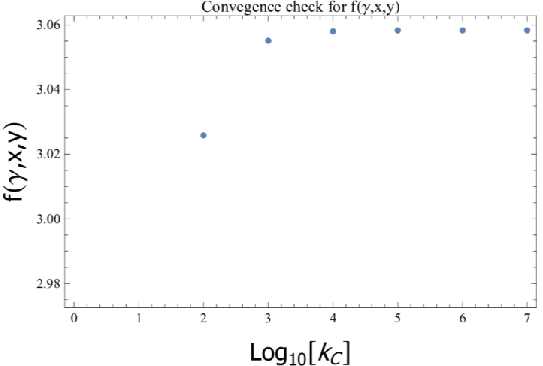
\includegraphics [width =0.7 \linewidth]{LHY_converge.pdf}
\end{center}
\caption[Convergence test of $f(\gamma ,x,y)$]{Convergence test of $f(\gamma ,x,y)$}  
\label{LHY_converge}
\end{figure}

% Minardi approximation
Now, we calculate $f(\gamma ,x,y)$ numerically for our Rb-Na Bose mixture system. First we do this integration and check its convergence. We plot $f(\gamma ,x,y)$ with increasing upper bound of integration $k_C$ to test its convergence, as shown in Fig. \ref{LHY_converge}. We can say that integration up to order of 6 has converged. Then, we calculate $f(\gamma ,x,y)$ with different $x$, i.e. with different B-field. Compare with Minardi's approximation
\cite{Minardi2019}, where they propose a analytical approximation which will be more convenient for deriving GPE with LHY correction. Here is the formula:
\begin{equation}
f(z,u=1,x)\simeq \left(1+z^{3/5}x\right)^{5/2}
\end{equation}
where
\begin{equation}
z=m_2/m_1, x=\frac{g_{22}n_2}{g_{11}n_1},u=\frac{g_{12}^2}{g_{11}g_{22}}
\end{equation}
Here, $u$ is set to be 1, because we only consider the case with near-zero MF energy, i.e. $g_{12}\approx\sqrt{g_{11}g_{22}}$ Now, we compare the numerical solution with the Minardi's approximation. Plot of List of f($\gamma $,x,y) for numerical one and Minardi's approximation. we can see that, there are mainly several percentage error by using this formula. And the maximum error is about 15$\%$. So, keep this error in mind about the LHY energy. (as show in Fig. \ref{LHY_Minardi})

% LHY_Minardi (done 2021-10-29 22:04:30)
\begin{figure}[htb]
\begin{center}
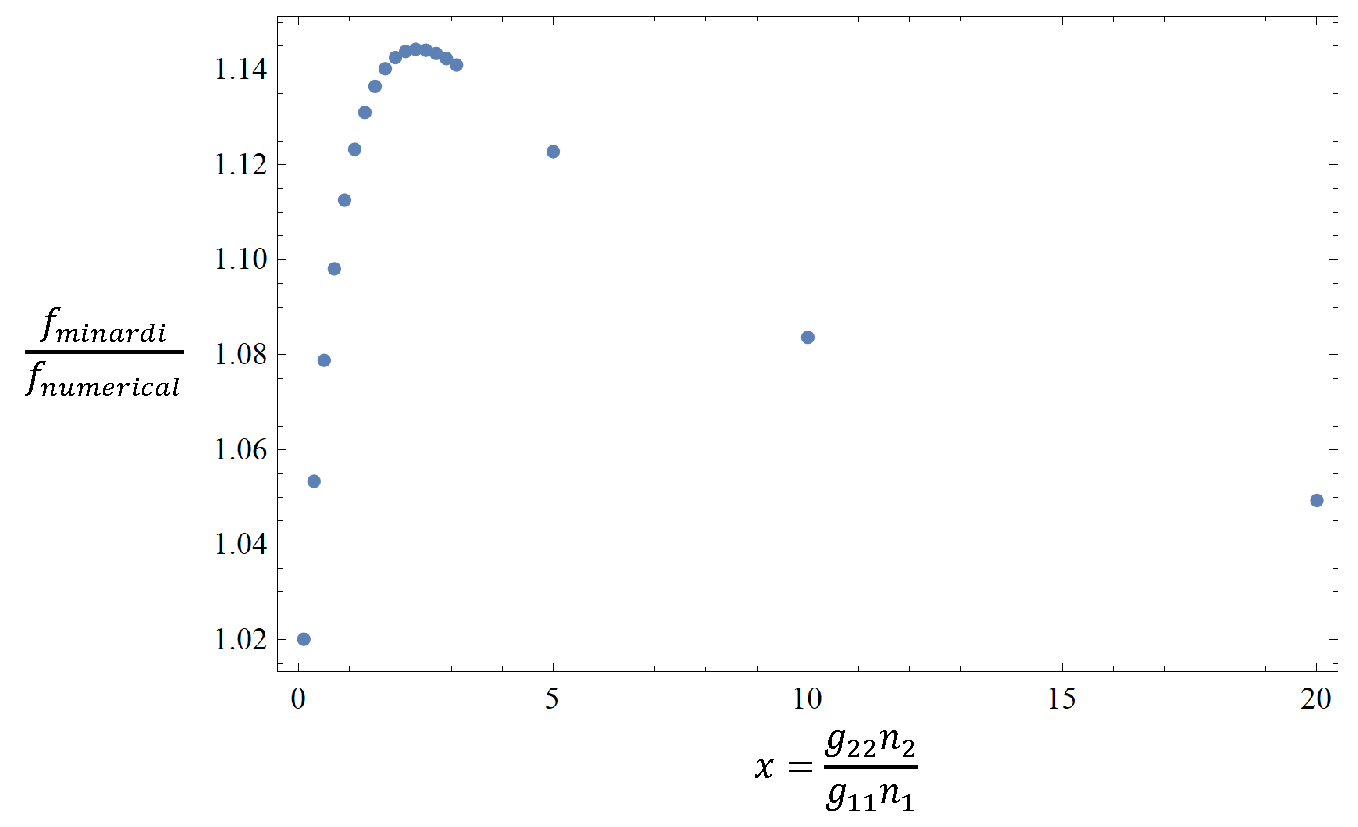
\includegraphics [width =0.85 \linewidth]{LHY_Minardi.pdf}
\end{center}
\caption[Compare the numerical solution and Minardi's approximation of $f(\gamma ,x,y)$]{Compare the numerical solution and Minardi's approximation of $f(\gamma ,x,y)$. The maxinum deviation is about 15\% when $g_{22}n_2/g_{11}n_1$ is around 2.}
\label{LHY_Minardi}
\end{figure}

% why we adopt this approximation (done 2021-10-29 22:04:52)
The subsequent GPE calculation requires a considerable amount of calculation. For example, for a 3D sample, if we split $2^7$ in each direction, then the calculation amount is to give an estimate. If the above infinite integral method is used to calculate the local of each grid LHY correction, then the amount of calculation will be huge. Therefore, if there is an analytical expression that can calculate the LHY correction, the amount of calculation will be significantly reduced. So Minardi approximation is a good starting point.

\subsection{Derivation of GPE for single species BEC}

% Derivation of single BEC GPE
First, we assume the many-body wave function is a product state
\begin{equation}
\Psi \left(\overset{\rightharpoonup }{r}_1,\overset{\rightharpoonup }{r}_2,\ldots  ,\overset{\rightharpoonup }{r}_N\right)=\sum _{i=1}^N \psi \left(\overset{\rightharpoonup}{r}_i\right)
\end{equation}
Then, we have
\begin{equation}
E\left(\psi ,\psi ^*\right)=N\int dr^3\left(\frac{\hbar ^2}{2m}\left| \nabla \psi (r)\right| ^2+V(r)\left| \psi (r)\right| ^2+\frac{1}{2}N g\left|\psi (r)\right| ^4\right)
\end{equation}
define the Variation
\begin{equation}
X\left(\psi ,\psi ^*\right)=E\left(\psi ,\psi ^*\right)-\mu  N\int dr^3\left| \psi (r)\right| ^2
\end{equation}
take the variation of $X\left(\psi ,\psi ^*\right)$, we have
\begin{equation}
\begin{split}
\delta  X\left(\psi ,\psi ^*\right)&=N\int dr^3\left[\frac{\hbar ^2}{2m}\left(\nabla \psi ^*(r)\nabla \delta \psi (r)+\nabla \psi (r)\nabla \delta \psi ^*(r)\right)\right.\\
&\left.\qquad\qquad+(V(r)-\mu )\left(\psi ^*(r)\delta  \psi (r)+\psi (r)\delta  \psi ^*(r) \right)\right.\\
&\left.\qquad\qquad+N g\left(\psi ^2(r)\delta  \psi ^*(r)+\psi ^{*2}(r)\delta\psi (r)\right)\right]\\
&=N\int dr^3\left[\frac{\hbar ^2}{2m}\left(\nabla \psi (r)\nabla \delta \psi ^*(r)\right)+(V(r)-\mu )\left(\psi (r)\delta  \psi ^*(r) \right)\right.\\
&\left.\qquad\qquad+N g\left(\psi^2(r)\psi ^*(r)\delta  \psi ^*(r)\right)\right]+c.c.
\end{split}
\end{equation}
for the first part, by using integrating by part method:
\begin{equation}
\begin{split}
\int dr^3\left(\nabla \psi (r)\nabla \delta \psi ^*(r)\right)&=\delta \psi ^*(r)\nabla \psi (r)|_0^{\infty }-\int dr^3\left(\nabla ^2\psi (r)\delta
\psi ^*(r)\right)\\
&=\int dr^3\left(-\nabla ^2\psi (r)\right)\delta \psi ^*(r)
\end{split}
\end{equation}
Then, take the variance to be zero, we have GPE
\begin{equation}
\begin{split}
-\frac{\hbar ^2}{2m}\left(\nabla ^2\psi (r)\right)+(V(r)-\mu )\psi (r)+N g\left(\psi ^2(r)\psi ^*(r)\right)=0\\
-\frac{\hbar ^2}{2m}\left(\nabla^2\psi^*(r)\right)+(V(r)-\mu)\psi ^*(r)+N g\left(\psi ^{*2}(r)\psi (r)\right)=0
\end{split}
\end{equation}

\subsection{Derivation of extended GPE for double species}
First, we assume the many-body wave function is a product state
\begin{equation}
\Psi \left(\overset{\rightharpoonup }{r}_1,\overset{\rightharpoonup }{r}_2,\ldots  ,\overset{\rightharpoonup }{r}_N\right)=\sum _{i=1}^N \psi \left(\overset{\rightharpoonup
}{r}_i\right)
\end{equation}
Then, we have
\begin{equation}
\begin{split}
E\left(\psi ,\psi ^*\right)=&N\int dr^3\left[\frac{\hbar ^2}{2m}\left(\nabla \psi ^*(r)\nabla \psi (r)\right)+V(r)\left(\psi ^*(r)\psi (r)\right)\right.\\
&\left.+\frac{1}{2}N g\left(\psi ^*(r)\psi (r)\right)^2+C \left(\psi ^*(r)\psi (r)\right)^{5/2}\right]
\end{split}
\end{equation}
define the Variation
\begin{equation}
X\left(\psi ,\psi ^*\right)=E\left(\psi ,\psi ^*\right)-\mu  N\int dr^3\left(\psi ^*(r)\psi (r)\right)
\end{equation}
take the variation of $X\left(\psi ,\psi ^*\right)$, we have
\begin{equation}
\begin{split}
\delta  X\left(\psi ,\psi ^*\right)&=N\int dr^3\left[\frac{\hbar ^2}{2m}\left(\nabla ^2\psi (r)\delta \psi ^*(r)\right)+(V(r)-\mu )\left(\psi (r)\delta\psi ^*(r) \right)\right.\\
&\left.+N g\left(\psi ^2(r)\psi ^*(r)\delta \psi ^*(r)\right)+\frac{5C}{2}(\psi (r))^{5/2}\left(\psi ^*(r)\right)^{3/2}\delta \psi ^*(r)\right]+c.c.
\end{split}
\end{equation}
where C is constants which already expressed the Last Part.
thus, we have eGPE
\begin{equation}
-\frac{\hbar ^2}{2m}\nabla ^2\psi (r)+(V(r)-\mu )\psi (r)+N g\left|\psi (r)\right|^2\psi(r)+\frac{5C}{2}\left|\psi (r)\right|^3\psi (r)=0
\end{equation}

% double species BEC
First, we assume the many-body wave function is a product state
\begin{equation}
\Psi \left(\overset{\rightharpoonup }{r}_1,\overset{\rightharpoonup }{r}_2,\ldots  ,\overset{\rightharpoonup }{r}_N\right)=\sum _{i=1}^N \psi _1\left(\overset{\rightharpoonup
}{r}_i\right)\sum _{i=1}^N \psi _2\left(\overset{\rightharpoonup }{r}_i\right)
\end{equation}
Then, we have
\begin{equation}
E\left(\psi _1,\psi _1{}^*,\psi _2,\psi _2{}^*\right)=\int dr^3\left(
\begin{array}{cc}
 \psi _1^* & \psi _2^* \\
\end{array}
\right).\left(
\begin{array}{cc}
 \mathcal{H}_{11} & \mathcal{H}_{12} \\
 \mathcal{H}_{21} & \mathcal{H}_{22} \\
\end{array}
\right).\left(
\begin{array}{c}
 \psi _1 \\
 \psi _2 \\
\end{array}
\right)+E_{\text{LHY}}
\end{equation}

where $\mathcal{H}_{ij}$ represent the Hamiltonian density of fields
\begin{equation}
\begin{split}
\mathcal{H}_{11}&=N_1\left(\frac{\hbar ^2}{2m_1}(\nabla )^2+V_1(r)+\frac{1}{2}N_1g_{11}\left(\psi _1{}^*(r)\psi _1(r)\right)\right)\\
\mathcal{H}_{22}&=N_2\left(\frac{\hbar ^2}{2m_2}(\nabla )^2+V_2(r)+\frac{1}{2}N_2g_{22}\left(\psi _2{}^*(r)\psi _2(r)\right){}^2\right)\\
\mathcal{H}_{12}&=\mathcal{H}_{21}^{\dagger }=N_1N_2g_{12}\left(\psi _1{}^*(r)\psi _1(r)\right)\left(\psi _2{}^*(r)\psi _2(r)\right)
\end{split}
\end{equation}
and LHY term has been expressed in the last part.
define the Variation
\begin{equation}
X\left(\psi ,\psi ^*\right)=E\left(\psi ,\psi ^*\right)-\mu _1 N_1\int dr^3\left(\psi _1{}^*(r)\psi _1(r)\right)-\mu _2 N_2\int dr^3\left(\psi
_2{}^*(r)\psi _2(r)\right)
\end{equation}

Finally, we have eGPE for 
\begin{equation}
\begin{split}
i \hbar \frac{\partial\psi_1}{\partial t}=\left(-\frac{\hbar^2\nabla^2}{2m_1}+V_1+g_{11}n_1+g_{12}n_2+\frac{\delta  \mathcal{E}_{\text{LHY}}}{\delta n_1}\right)\psi _1\\
i \hbar \frac{\partial \psi _2}{\partial t}=\left(-\frac{\hbar ^2\nabla ^2}{2m_2}+V_2+g_{22}n_2+g_{12}n_1+\frac{\delta  \mathcal{E}_{\text{LHY}}}{\delta n_2}\right)\psi _2
\end{split}
\end{equation}

\subsection{eGPE for GPELAB with Minardi approximation}

\begin{equation}
\begin{split}
i \hbar \frac{\partial\psi_1}{\partial t}=\left(-\frac{\hbar^2\nabla^2}{2m_1}+V_1+g_{11}n_1+g_{12}n_2+\frac{\delta  \mathcal{E}_{\text{LHY}}}{\delta n_1}\right)\psi _1\\
i \hbar \frac{\partial \psi _2}{\partial t}=\left(-\frac{\hbar ^2\nabla ^2}{2m_2}+V_2+g_{22}n_2+g_{12}n_1+\frac{\delta  \mathcal{E}_{\text{LHY}}}{\delta n_2}\right)\psi _2
\end{split}
\end{equation}
where$n_i=N_i\psi _i^*\psi _i=N_i|\psi _i|^2$ and 
\begin{equation}
\frac{\delta  \mathcal{E}_{\text{LHY}}}{\delta  n_1}=\frac{8}{15\pi^2}\frac{m_1^{3/2}\left(g_{11}\right){}^{5/2}n_1^{1/2}}{\hbar^3}\left(\frac{5}{2}n_1f(\gamma,x,y)-\frac{g_{22}n_2}{g_{11}}\frac{\partial f(\gamma ,x,y)}{\partial y}\right)
\end{equation}
\begin{equation}
\frac{\delta  \mathcal{E}_{\text{LHY}}}{\delta  n_2}=\frac{8}{15\pi^2}\frac{m_1^{3/2}\left(g_{11}\right){}^{3/2}g_{22}n_1^{3/2}}{\hbar ^3}\frac{\partial
f(\gamma ,x,y)}{\partial y}
\end{equation}
if we using the approximation formula, we have
\begin{equation}
\mathcal{E}_{\text{LHY}}=\frac{8}{15\pi ^2}\frac{m_1^{3/2}\left(g_{11}n_1\right){}^{5/2}}{\hbar ^3}\left(1+\gamma ^{3/5}y\right)^{5/2}
\end{equation}
Then, 
\begin{equation}
\begin{split}
\frac{\delta  \mathcal{E}_{\text{LHY}}}{\delta  n_1}&=\frac{8}{15\pi^2}\frac{m_1^{3/2}\left(g_{11}\right){}^{5/2}n_1^{1/2}}{\hbar^3}\left(\frac{5}{2}n_1\left(1+\gamma^{3/5}y\right){}^{5/2}-\frac{5}{2}\frac{g_{22}n_2}{g_{11}}\left(1+\gamma ^{3/5}y\right)^{3/2}\gamma ^{3/5}\right)\\
&=\frac{4}{3\pi^2}\frac{m_1^{3/2}\left(g_{11}\right){}^{5/2}n_1^{3/2}}{\hbar^3}\left(1+\gamma^{3/5}y\right)^{3/2}
\end{split}
\end{equation}
\begin{equation}
\begin{split}
\frac{\delta  \mathcal{E}_{\text{LHY}}}{\delta n_2}&=\frac{8}{15\pi^2}\frac{m_1^{3/2}\left(g_{11}\right){}^{3/2}g_{22}n_1^{3/2}}{\hbar^3}\frac{5}{2}\left(1+\gamma^{3/5}y\right)^{3/2}\gamma ^{3/5}\\
&=\frac{4}{3\pi^2}\frac{\gamma^{3/5}m_1^{3/2}\left(g_{11}\right){}^{3/2}g_{22}n_1^{3/2}}{\hbar^3}\left(1+\gamma ^{3/5}y\right)^{3/2}
\end{split}
\end{equation}
Finally, we have extended GPE as
\begin{equation}
\begin{split}
i \hbar \frac{\partial \psi _1}{\partial t}=\left(-\frac{\hbar ^2\nabla ^2}{2m_1}+V_1+g_{11}n_1+g_{12}n_2+\frac{4}{3\pi ^2}\frac{g_{11}m_1^{3/5}}{\hbar
^3}\left(g_{11}n_1m_1^{3/5}+g_{22}n_2m_2^{3/5}\right){}^{3/2}\right)\psi _1\\
i \hbar \frac{\partial \psi _2}{\partial t}=\left(-\frac{\hbar ^2\nabla ^2}{2m_2}+V_2+g_{22}n_2+g_{12}n_1+\frac{4}{3\pi ^2}\frac{g_{22}m_2^{3/5}}{\hbar
^3}\left(g_{11}n_1m_1^{3/5}+g_{22}n_2m_2^{3/5}\right){}^{3/2}\right)\psi _2
\end{split}
\end{equation}
Now, we need do Dimension-Reduction, 
\begin{equation}
\begin{split}
i \frac{\partial \Psi _1}{\partial T}&=\left[-\frac{m\pmb{\nabla }^2}{2m_1}+\frac{V_1}{\hbar  \omega }+4\pi  \frac{m}{m_1}\frac{ N_1a_{11}}{a}\Psi_1^*\Psi _1+2\pi \frac{ m }{m_{12}}\frac{N_2a_{12}}{a}\Psi _2^*\Psi _2\right.\\
&\left.+\frac{128\pi ^{1/2} }{3} \frac{a_{11}}{a}\left(\frac{m}{m_1}\right){}^{2/5}\left(\frac{N_1a_{11}}{a}\left(\frac{m}{m_1}\right){}^{2/5}\Psi _1^*\Psi _1\right.\right.\\
&\left.\left.+ \frac{N_2a_{22}}{a}\left(\frac{m}{m_2}\right){}^{2/5}\Psi _2^*\Psi _2\right){}^{3/2}\right]\Psi_1\\
i \frac{\partial \Psi _2}{\partial T}&=\left[-\frac{m\pmb{\nabla }^2}{2m_2}+\frac{V_2}{\hbar  \omega }+4\pi  \frac{m}{m_2}\frac{\text{  }N_2a_{22}}{a}\Psi_2^*\Psi _2+2\pi \frac{ m }{m_{12}}\frac{N_1a_{12}}{a}\Psi _1^*\Psi _1\right.\\
&\left.+\frac{128\pi ^{1/2} }{3}\frac{a_{22}}{a}\left(\frac{m}{m_2}\right){}^{2/5}\left(\frac{N_1a_{11}}{a}\left(\frac{m}{m_1}\right){}^{2/5}\Psi _1^*\Psi _1\right.\right.\\
&\left.\left.+ \frac{N_2a_{22}}{a}\left(\frac{m}{m_2}\right){}^{2/5}\Psi _2^*\Psi _2\right){}^{3/2}\right]\Psi_2
\end{split}
\end{equation}
where we set $V_1$ and $V_2$ as harmonic trap, and it gives the characteristic length and time. Actually, this characteristic length and time can be arbitrary.
\begin{equation}
\begin{split}
g_{11}=\frac{4\pi  \hbar ^2a_{11}}{m_1}, g_{22}=\frac{4\pi  \hbar ^2a_{22}}{m_2}, g_{12}=\frac{2\pi  \hbar ^2a_{12}}{m_{12}}, m_{12}=\frac{m_1m_2}{m_1+m_2}\\
T=\omega  t, \overset{\rightharpoonup }{R}=\left.\overset{\rightharpoonup }{r}\right/a, \Psi =\psi  a^{3/2}, a=\sqrt{\frac{\hbar }{m \omega }}
\end{split}
\end{equation}
By the way, we can calculate the Nonlinear-Energy function. (Just for fun, not for GPELAB)
Recall LHY energy term
\begin{equation}
\begin{split}
\mathcal{E}_{\text{LHY}}=\frac{8}{15\pi ^2}\frac{m_1^{3/2}\left(g_{11}n_1\right){}^{5/2}}{\hbar ^3}\left(1+\left(\frac{m_2}{m_1}\right){}^{3/5}\frac{g_{22}n_2}{g_{11}n_1}\right){}^{5/2}\\
=\frac{256\sqrt{\pi }\hbar ^2}{15}\left(m_1^{-2/5}a_{11}n_1+m_2^{-2/5}a_{22}n_2\right){}^{5/2}
\end{split}
\end{equation}
Do Dimension-Reduction, we have
\begin{equation}
\frac{\mathcal{E}_{\text{LHY}}}{\hbar\omega\left/a^3\right.}=\frac{256\pi^{1/2}}{15}\left(\frac{N_1a_{11}}{a}\left(\frac{m}{m_1}\right){}^{2/5}\Psi_1^*\Psi_1+\frac{N_2a_{22}}{a}\left(\frac{m}{m_2}\right){}^{2/5}\Psi _2^*\Psi _2\right){}^{5/2}
\end{equation}

\section{Na-Rb Hetero-nuclear quantum droplet}
\label{sec:droplet_experiment}

This section\footnote{This section is mainly from our paper \cite{guo2021leehuangyang}.} demonstrates our experiment study on the quantum droplet made of Na-Rb BEC mixture. Our experiment starts from an optically trapped double BEC of $^{23}$Na and $^{87}$Rb (denoted as species 1 and 2 hereafter, respectively) both prepared in their lowest-energy hyperfine Zeeman level $\ket{F = 1, m_F = 1}$~\cite{wang2015double}. To reveal the LHY effects, we focus on the near-zero MF region with $\delta g = g_{12} + \sqrt{g_{11} g_{22}} \approx 0$. Here $g_{ij} = 2\pi\hbar^2 a_{ij}/M_{ij}$ are the two-body interaction constants, with $a_{ij}$ the scattering lengths and $M_{ij}$ the reduced masses. To reach this regime, we use the Na-Rb Feshbach resonance at $B_0 = 347.648$~G to tune the Na-Rb scattering length. The scattering length is represented as $a_{12} = a_\text{bg}\big(1-\Delta/(B-B_0)\big)$ [upper panel of Fig.~\ref{fig1}(a)], with background scattering length $a_\text{bg} = 76.33a_0$ and resonance width $\Delta = 4.255$~G~\cite{wang2013observation}. Near $B_0$ the intraspecies scattering lengths $a_{11} = 60.05a_0$~\cite{Knoop2011} and $a_{22} = 100.13a_0$~\cite{Kempen2002} remain almost constant. 

%% add figure1 here
\begin{figure}[hbt]
\begin{center}
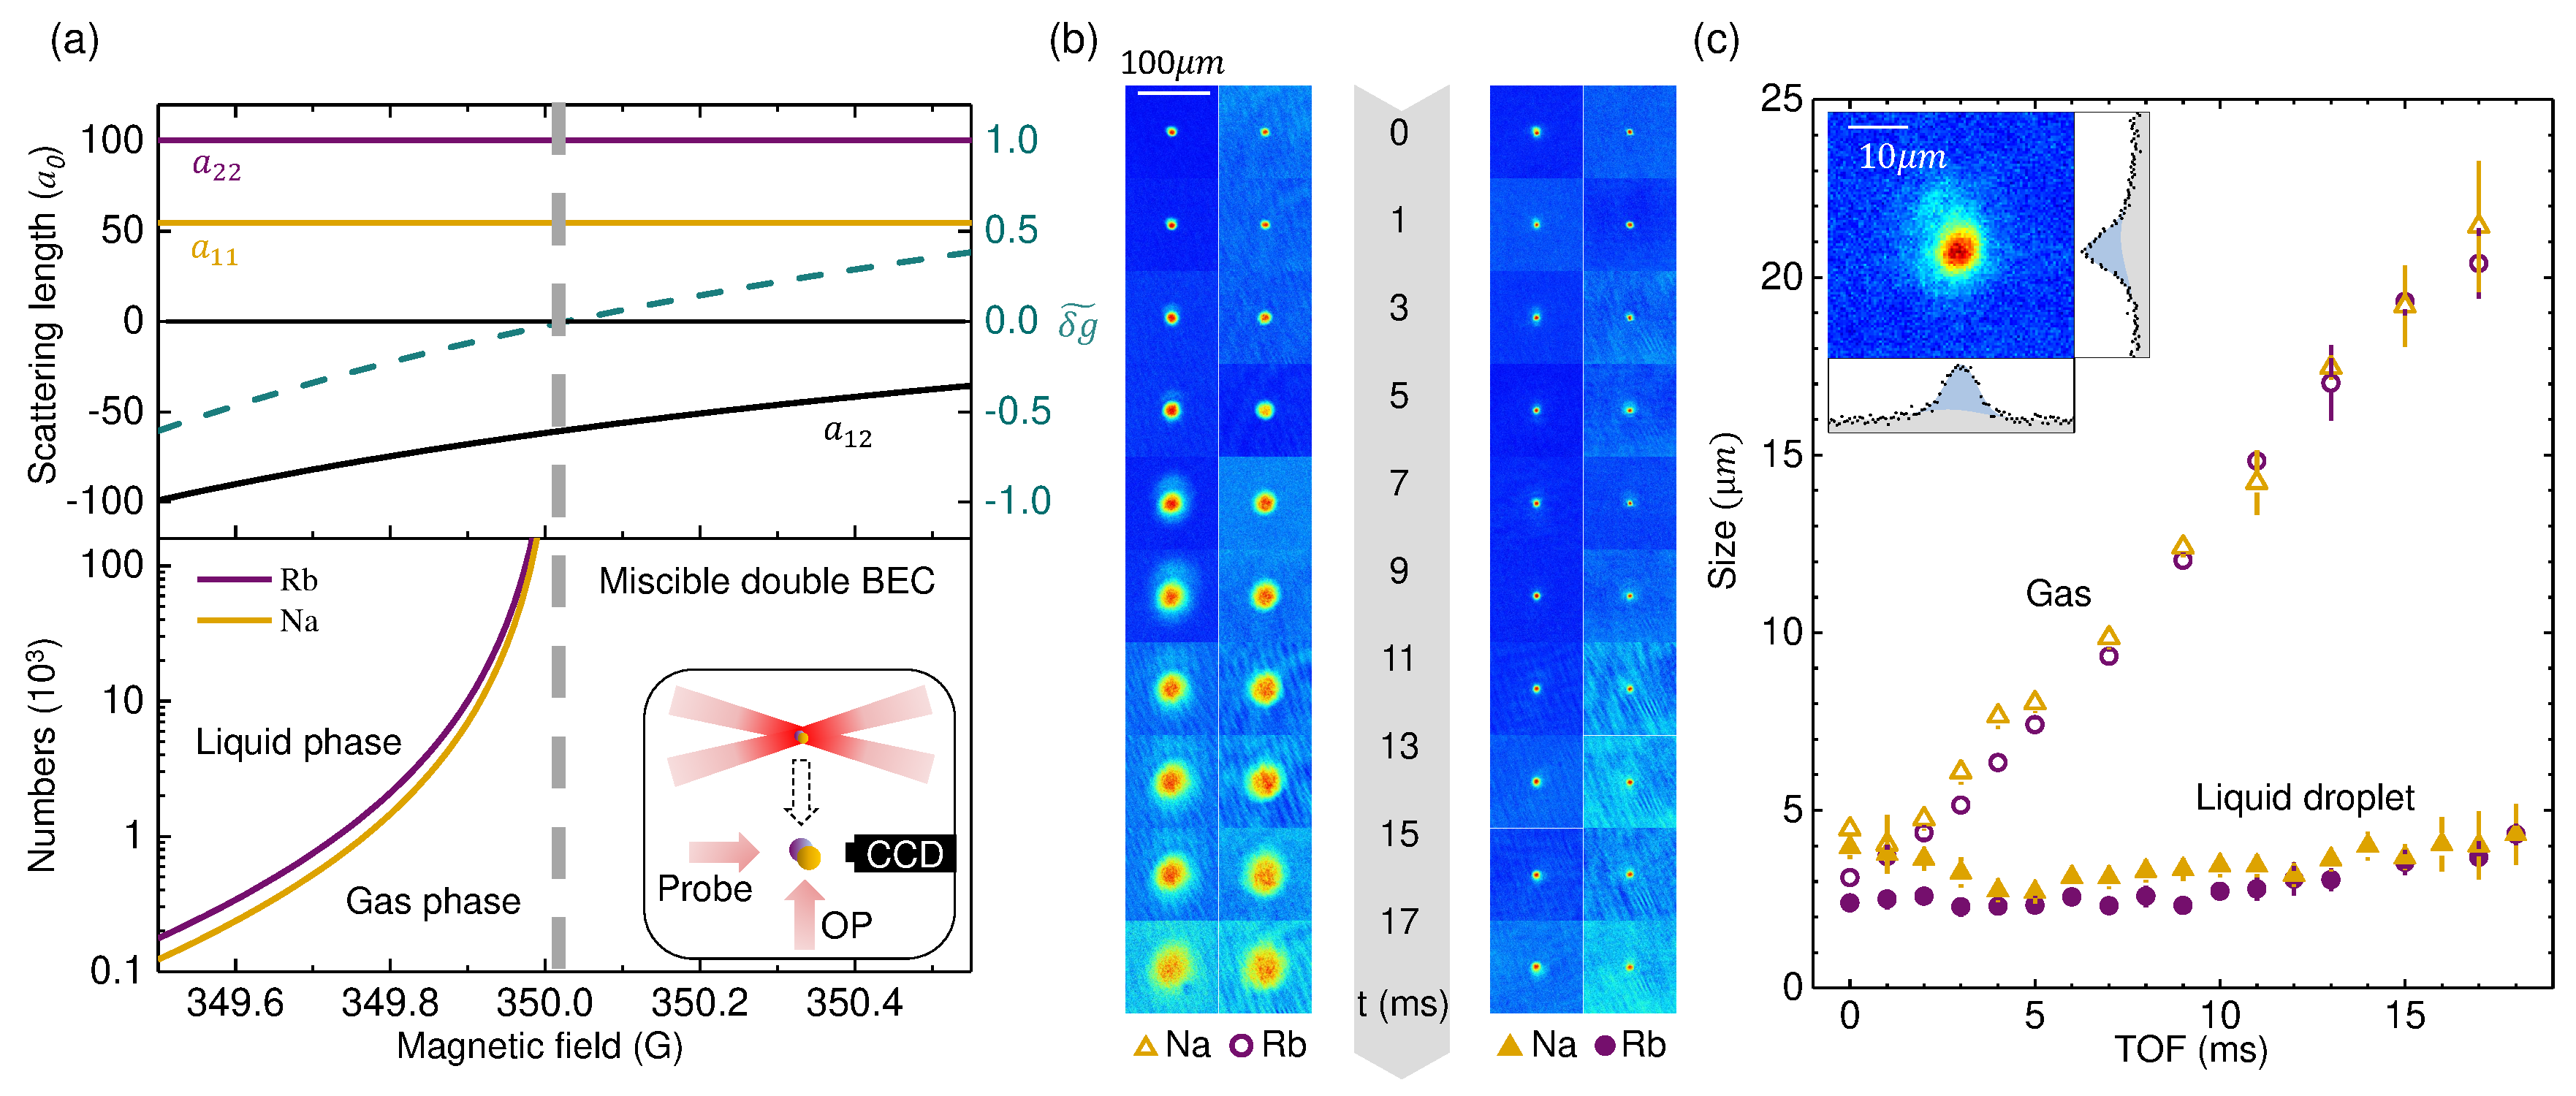
\includegraphics [width = \linewidth]{fig1.pdf}
\end{center}
\caption[Creation and detection of Na-Rb mixtures for investigating LHY effects]{Creation and detection of Na-Rb mixtures for investigating LHY effects. (a) In the upper panel, the purple, yellow, and black solid lines are scattering lengths between Na-Na($a_{11}$), Rb-Rb($a_{22}$) and Na-Rb($a_{12}$), respectively. The dashed green curve is $\widetilde{\delta g}$. The dashed vertical line indicates the magnetic field for $\widetilde{\delta g} = 0$. In the lower panel, the phase diagrams at different atomic numbers and magnetic fields are shown. Inset: schematic detection method of the droplet in free space. (b) Images of the mixture during the TOF expansion in the gas phase at 350.451 G (left) and the droplet phase at 349.849 G (right). (c) Cloud sizes obtained from (b) reveal the very different behaviors of the two phases. Data points for $^{87}$Rb are shown in purple, while those for $^{23}$Na are in yellow. Inset: in the droplet phase, 
bimodal distributions are observed for the cloud with excess atoms. A double Gaussian fitting is used to extract the droplet size in this case.
}
\label{fig1}
\end{figure}
%% add figure1 here

For convenience, we define a dimensionless parameter $\widetilde{\delta g} \equiv \delta g/\overline{g}$ to characterize the total $E_{\rm MF}$, with $\overline{g} = (g_{11}+g_{22})/2$. For the current system, the critical magnetic field for $\widetilde{\delta g} = 0$ (and also $\delta g= 0$) is $B_c = 349.978$~G, which corresponds to a critical interspecies scattering length $a^c_{12} = -63.1 a_0$. As shown in Fig.~\ref{fig1}(a) (lower panel), for each value of $\widetilde{\delta g} < 0$, the double BEC will undergo a transition from gas phase to droplet phase as the atom numbers are increased. With our atom numbers around $10^4$ for both species, the theory predicts an observation window for the droplet phase for $\widetilde{\delta g}$ from $-0.061$ to $-0.189$ (349.910 G to 349.780 G). For $\widetilde{\delta g}$ from 0 to $-0.061$, droplet formation is still possible but atom numbers much larger than currently available are needed.

\subsection{Experiment method and time sequence}

%imaging method
In the first experiment, we study the Na-Rb quantum droplet in free space by releasing the sample from the optical trap. We probe the system during the time of flight (TOF), as depicted in the inset of Fig.~\ref{fig1}(a). To probe the atoms in situ at each TOF, we implement a two-species high-field detection protocol which consists of a partial optical pumping process followed by standard absorption imaging on the cycling transitions~\cite{jia2020}. This partial imaging method is necessary as the droplets have very high optical depth and are difficult to detect directly~\cite{ramanathan2012partial,semeghini2018self}. Both the partial optical pumping and the absorption imaging are calibrated using standard methods~\cite{reinaudi2007strong,hueck2017calibrating}. The measured resolutions ($1/\sqrt{e}$ half Gaussian widths) of our imaging system are $0.6~\mu$m and $0.8~\mu$m for $^{23}$Na at 589 nm and $^{87}$Rb at 780 nm, respectively, which are just enough to resolve the droplet. To maintain the imaging resolutions, we mount the objective and the probe light optics on high-precision vertical translational stages to keep the optical axis of the imaging system always aligned with the droplet.

%experiment method and time sequence
Figure \ref{droplet_time_sequence} shows the time sequence we produce quantum droplet. While shutting down the optical trap provides a direct way of probing the droplet in free space, the non-adiabatic nature of the process can cause problems. Due to the confinement, the in-trap sample is smaller in size than the free-space droplet in its ground state, while the total energy of the system is much larger. In the worst scenario, the energy of the initial state upon release from the trap is larger then the energy barrier of the expansion and a stable droplet can never be formed. To mitigate this problem, the crossed optical dipole trap is configured in a nearly spherical shape with measured trap oscillation frequencies of 78 Hz (86 Hz) for $^{87}$Rb ($^{23}$Na). This is in accordance with the understanding that a quantum droplet with isotropic short-range interactions should be spherical in free space. In addition, a carefully designed magnetic field control sequence is used to improve the mode matching. These steps allow us to observe droplet formation reliably for $\widetilde{\delta g}$ from $-0.094$ to $-0.189$. However, for $\widetilde{\delta g}$ from $-0.061$ to $-0.094$, due to the smaller binding energy, droplets can be observed only by a more sophisticated mode-matching method, aided by fast magnetic field quenching at the instant of releasing the samples from the trap. For this method to work, the starting magnetic field must be selected carefully so that the size of the in-trap sample matches that of the free-space droplet at the end of the magnetic field quenching.

% time sequence
\begin{figure}[hbt]
\begin{center}
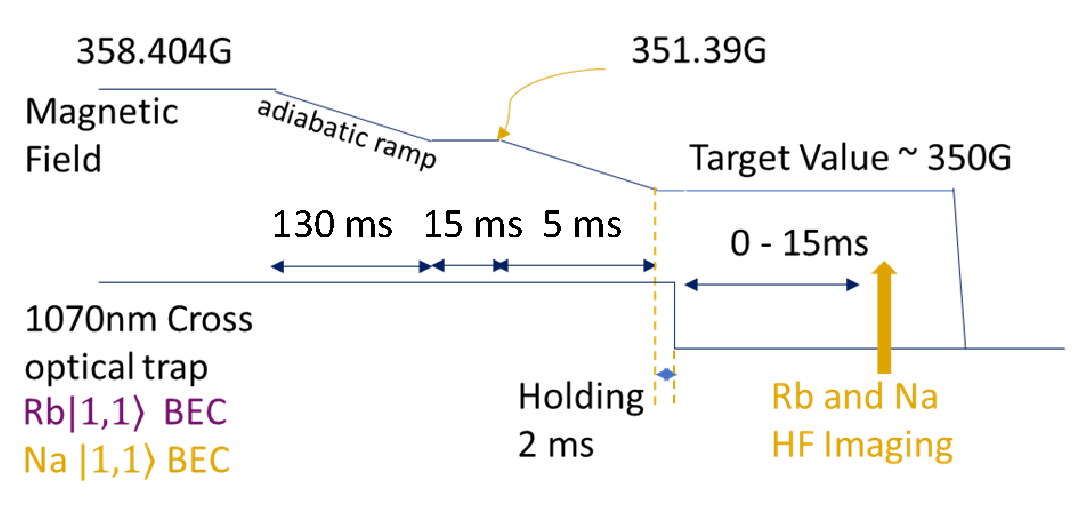
\includegraphics[width = 0.8\linewidth]{figures/droplet_time_sequence.pdf}
\end{center}
\caption[Time sequence for producing quantum droplet]{Time sequence for producing quantum droplet.}
\label{droplet_time_sequence}
\end{figure}

\subsection{observing non-expansion signal}

Figure~\ref{fig1}(b) shows a side-by-side comparison of the $^{23}$Na and $^{87}$Rb clouds in the gas phase and the droplet phase following the TOF. The signature self-bound behavior of the droplet can be observed clearly by comparing its dramatically different TOF expansion with that in the gas phase. For $\widetilde{\delta g}=-0.119$ (349.849 G), where the droplet phase is expected, the sizes of both clouds stay nearly the same during the TOF. For $\widetilde{\delta g}=+0.344$ (350.451 G), by contrast, the system remains in the gas phase, and the sizes increase steadily with TOF.

% fitting by Gaussian and double-Gaussian
To extract quantitative information, we fit the images with 2D Gaussian functions. In the droplet, the size should be the same for the two species; their densities and thus numbers should follow the ratio $N_{2}/N_{1} = \sqrt{g_{11}/g_{22}}=1.51$~\cite{petrov2015}. When this ratio is not maintained, the droplet part shows up as a dense central peak, and the excess atoms of one species appear as a much larger-sized and expanding gaseous background surrounding the droplet [inset of Fig.~\ref{fig1}(c)]. For this kind of ``bimodal'' distribution, the droplet parameters are extracted with a double 2D Gaussian fitting. Fig.~\ref{fig1}(c) shows the starkly different expansion behaviors in the droplet and the gas phases obtained from the images in Fig.~\ref{fig1}(b).

%% add figure2 here
\begin{figure}[htb]
\begin{center}
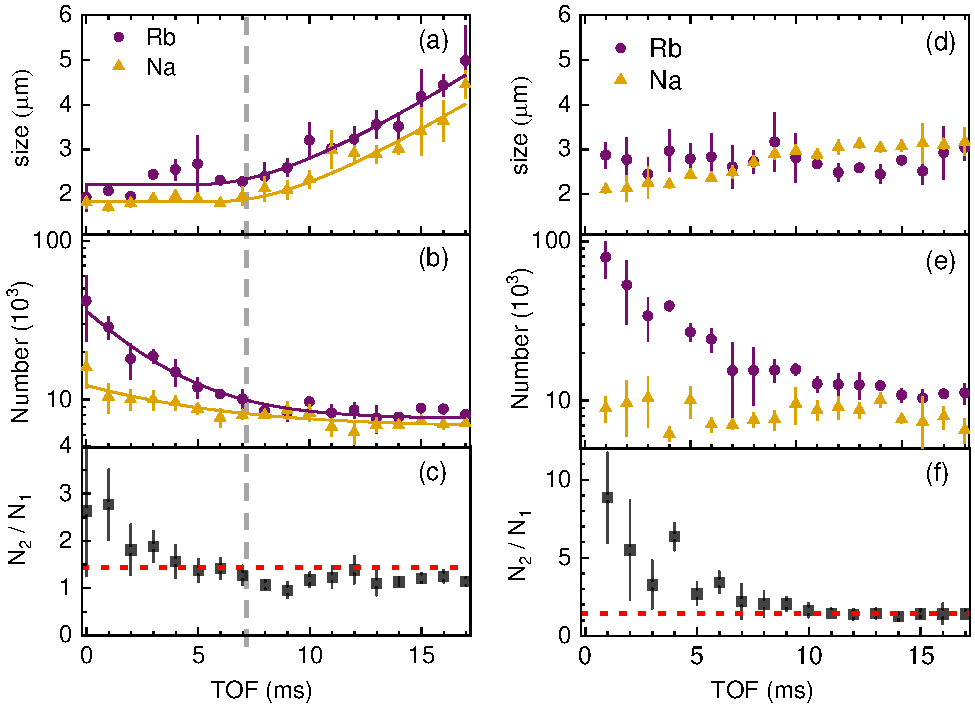
\includegraphics [width =0.95 \linewidth]{fig2.pdf}
\end{center}
\caption[Evolution of the Na-Rb droplet in free space]{Evolution of the Na-Rb droplet in free space. (a), (b), and (c) show the size, atom numbers, and the $^{87}$Rb to $^{23}$Na number ratio at $\widetilde{\delta g} = -0.116$ (349.852 G) following the TOF. The droplet is created by directly releasing the sample from the trap. The vertical bar marks the approximate time of the liquid-to-gas phase transition. (d), (e), and (f) show the evolution for the droplet created with the additional magnetic field quenching for $\widetilde{\delta g} = -0.089$ (349.880 G). The red dashed lines in (c) and (f) mark the theoretical number ratio $N_2/N_1=1.51$.}  
\label{fig2}
\end{figure}

%Explanation of Fig#2
%droplet formation
For the droplets formed by direct trap release from $\widetilde{\delta g} = -0.094$ to $-0.189$, we observe two distinctively different dynamics in the evolution of the $^{23}$Na and $^{87}$Rb samples during the TOF. As an example, Fig.~\ref{fig2}(a), (b) and (c) show the sizes, atom numbers, and number ratio of the droplet sample for $\widetilde{\delta g}=-0.116$ (349.852~G).
During the first 10 ms, the $^{23}$Na and $^{87}$Rb sizes increase very little, while atom losses are observed for both species.
Bimodal distributions are observed from 0 ms to 5 ms as the initial number ratio is far from 1.51. After 5 ms expansion, the gaseous atoms surrounding the droplet are already too dilute to be detected. 

%droplet to the gas phase transition
After about 10 ms, the sample sizes start to increase while the atom numbers stay nearly constant.
This is consistent with a phase transition from droplet to gas when the atom numbers are reduced to below the critical values [see Fig.~\ref{fig1}(a)]. We fit the size evolution empirically with $\sigma(t>t_0)=\sqrt{\sigma_0^2+v^2(t-t_0)^2}$ and $\sigma(t<t_0)=\sigma_0$, and obtain a lifetime in the droplet phase of about $t_0 = 7$ ms. Here $v$ is the expansion velocity of the gas-phase sample. Similarly, as illustrated in Fig.~\ref{fig2}(b), the critical atom numbers for the phase transition can be obtained by fitting the $^{23}$Na and $^{87}$Rb number evolution data with an 
exponential decay function with the critical number as the offset.

For several values of $\widetilde{\delta g}$ between $-0.061$ and $-0.094$, we have created longer-lived droplets by the magnetic field quenching method. As shown in Fig.~\ref{fig2}(d), (e) and (f), during the accessible TOF, the droplet size stays nearly the same although number losses are still observed. After 10 ms, the number ratio becomes close to 1.51 and the number loss slows down significantly. As the lifetime is longer than the usable TOF of 18 ms, we have not been able to measure the real lifetime and the critical numbers in this range of $\widetilde{\delta g}$. More detailed investigations, e.g., by levitating the droplet, are warranted in the near future.

\subsection{Characterization of liquid-gas phase transition}

Figure~\ref{fig3} shows the critical $^{23}$Na and $^{87}$Rb atom numbers for $\widetilde{\delta g}$ from $-0.146$ to $-0.247$. Although the range of $\widetilde{\delta g}$ is small, a four-fold change in the measured critical numbers is observed. The critical numbers calculated using coupled eGPEs with the LHY term included (dashed curves) show large discrepancies with the measurements. The agreement is greatly improved by also including the small post-compensation residual magnetic field gradient in the eGPEs (solid curves); the additional term nearly doubles  the critical numbers. This can be understood from the different magnetic dipole moments and masses of $^{23}$Na and $^{87}$Rb, which cause their centers of mass to separate in a magnetic field gradient. This decreases the density overlap and lowers the attractive interspecies mean-field energy while leaving the intraspecies energy nearly intact. Effectively, this increases the critical numbers compared to the ideal case of zero gradient.

%% add figure3 here
\begin{figure}[htb]
\begin{center}
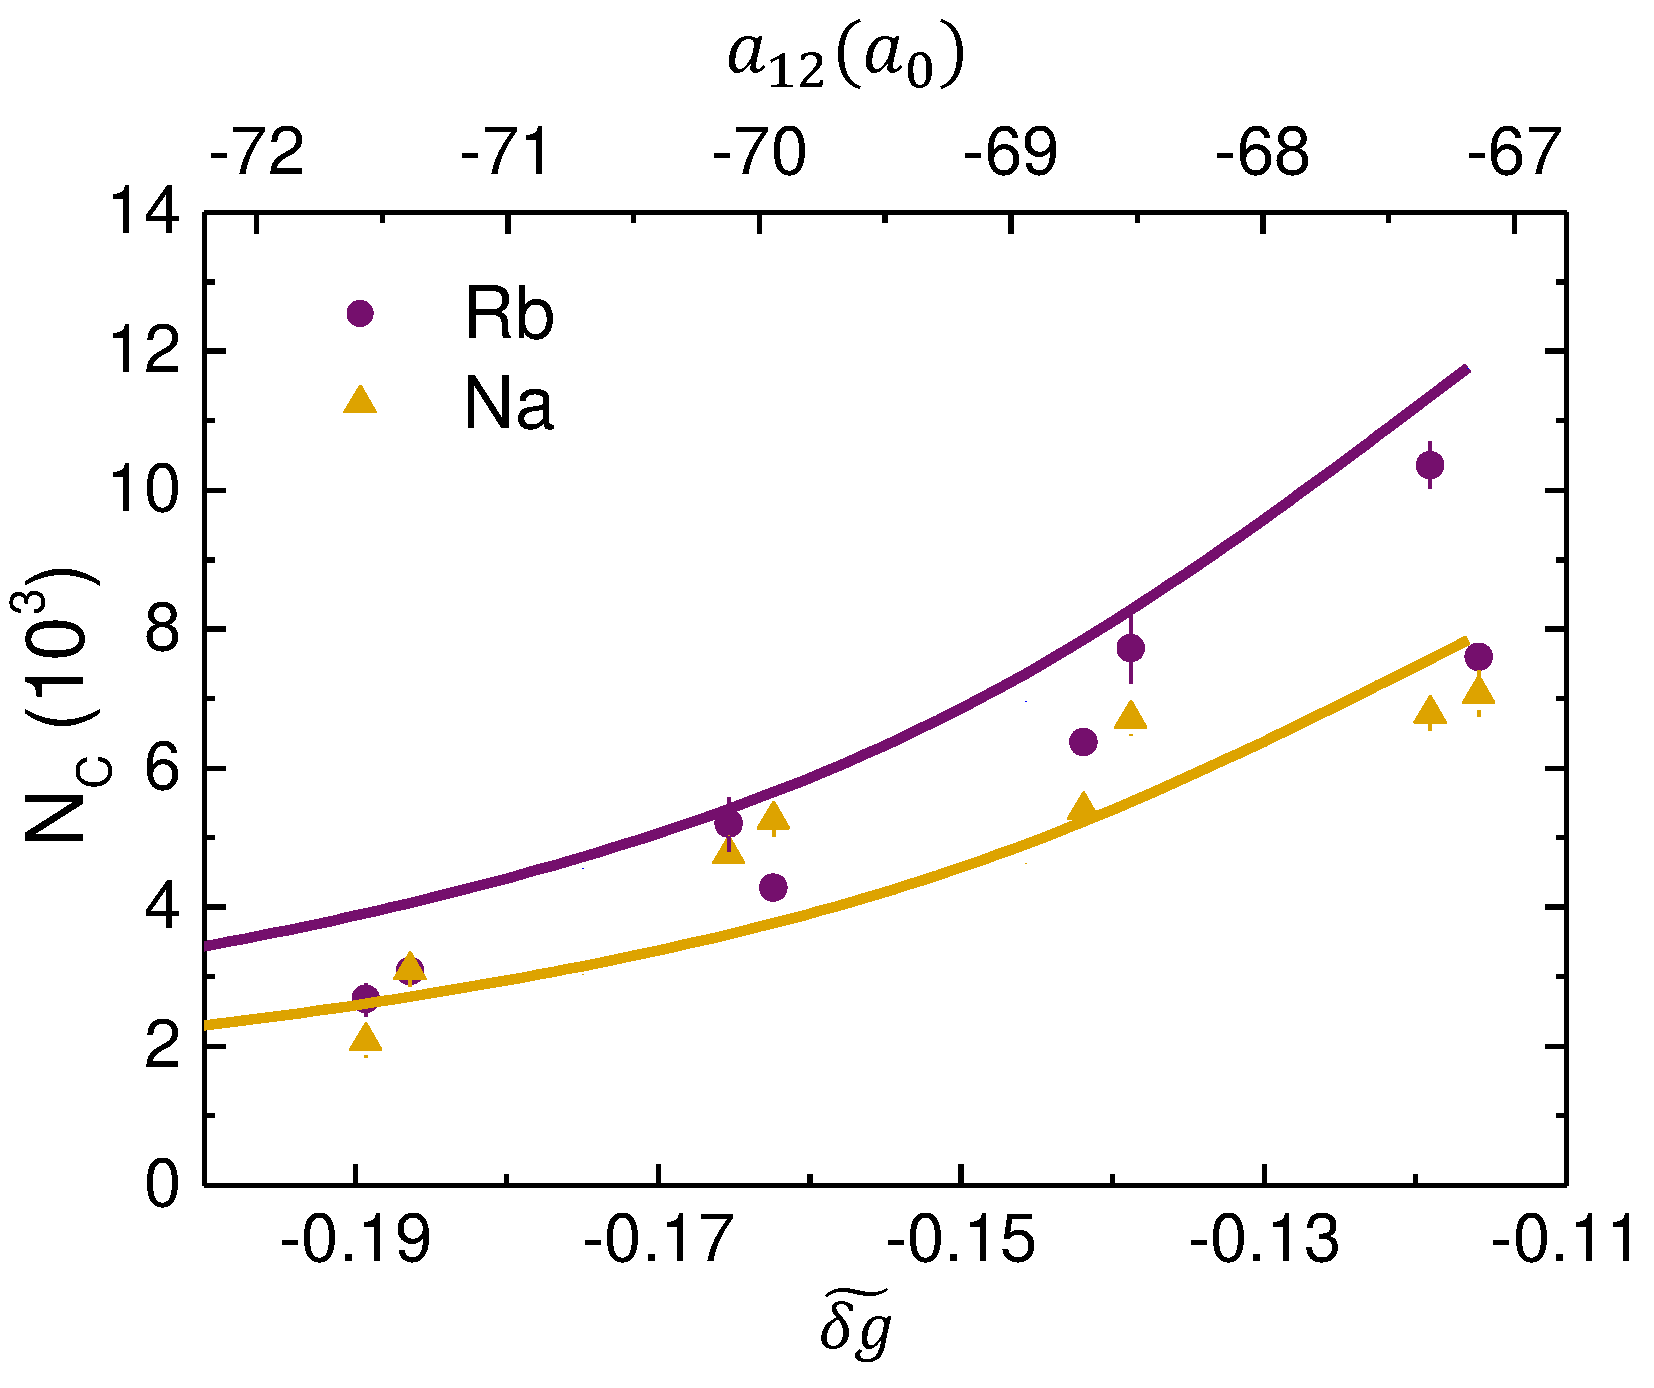
\includegraphics [width =0.85 \linewidth]{fig3.pdf}
\end{center}
\caption[Critical atom numbers for the liquid-to-gas phase transition as a function of $\widetilde{\delta g}$]{Critical atom numbers for the liquid-to-gas phase transition as a function of $\widetilde{\delta g}$. The solid lines are calculated from coupled eGPEs with the residual magnetic field gradient included.}
\label{fig3}
\end{figure}
%% add figure3 here

% about loss
A major cause of the atom losses is three-body recombination as a result of the high number densities in the droplet~\cite{cabrera2018quantum,semeghini2018self,DErrico2019}. For droplets with $\widetilde{\delta g}$ from $-0.094$ to $-0.189$, another possible loss mechanism is self-evaporation due to the imperfect matching between in-trap and free-space modes~\cite{Ferioli2020}. The short lifetimes in this region are the combined result of these loss mechanisms. In contrast, the droplet at $\widetilde{\delta g} = -0.089$ [see Fig.~\ref{fig2}(d), (e), and (f)] has relatively lower number densities and is formed with nearly optimal mode matching, and is thus longer lived. Nevertheless, for both cases, the stabilized number ratios after 10 ms TOF are very close to 1.51 despite the different creation procedures and the large initial number mismatches [Fig.~\ref{fig2}(c) and (f)].

\section{Lee-Huang-Yang gas}
\label{sec:LHY_gas}

We now turn to the gas-phase double BEC and release the sample directly from the trap (without the additional magnetic field quenching) for $\widetilde{\delta g}$ from +0.344 to $-0.094$. To characterize the LHY effect, we measure the release energy $E_{\rm rel}=E_{\rm kin}+E_{\rm int}$ from the TOF expansion~\cite{Holland1997,Mewes1996}. Here $E_\text{\rm kin}$ is the quantum pressure and $E_{\rm int}=E_{\rm MF}+E_{\rm LHY}$ is the total interaction energy. When $E_{\rm MF}$ is tuned to zero, $E_{\rm LHY}$ becomes the only interaction term in $E_{\rm rel}$. For negative $E_{\rm MF}$, the fact that the sample expands rather than collapses is also a direct manifestation of the LHY effect.

When we using TOF measurement on condensate from a harmonic trap, we lose the trap energy suddenly and the kinetic energy (quantum pressure) and the interaction energy converts to kinetic energy of motion after long-time evolution. So, we have the release energy
\begin{equation}
E_{\text{release}}=E_{\text{kin}}+E_{\text{MF}}=N \hbar  \omega _0\left(\frac{3}{4}\frac{1}{w^2}+\frac{1}{\sqrt{2\pi }}\frac{a_SN}{a_{\text{ho}}}\frac{1}{w^3}\right)
\end{equation}
put the numerical solution of $w$ into the release energy, we have for $g=0 \text{case}$, we have $E_{\text{release}}=\frac{3}{4}\hbar \omega _0$ With increasing $\chi$, we have larger size (larger $w$), and finally, when reach $\chi >>1$ limit, we turn to the Thomas-Fermi limit.

\subsection{Expansion of gas phase sample and Release energy}
%introduce the LHY gas, explain the difference between liquid droplet and LHY gas
In the previous sections, we describe a liquid phase droplet sample made of $^{23}\rm Na$--$^{87}\rm Rb$ BEC mixture. Now we turn to study the gas phase (LHY gas) of this mixture, in which the Lee-Huang-Yang effects still play an important role. The mainly difference between a droplet and a LHY gas sample is whether the kinetic energy dominates the Hamiltonian. For droplet sample, the competition mainly comes from the attractive mean-field term and the repulsive LHY term. When the atomic number drops down, and both mean-field and LHY energy goes down, finally the kinetic energy gets not negligible. After the balance point of density disappeared, as we describe about the liquid-gas phase transition, the sample turns to a gas-phase sample.

by directly releasing the sample from the trap for $\widetilde{\delta g}$ from +0.322 to -0.146.
To characterize the LHY effect in this situation, we measure the release energy $E_{\rm rel}=E_{\rm kin}+E_{\rm int}$ from the TOF expansion~\cite{Holland1997,Mewes1996}. Here $E_\text{\rm kin}$ is the quantum pressure and $E_{\rm int}=E_{\rm MF}+E_{\rm LHY}$ is the total interaction energy. When $E_{\rm MF}$ is tuned to zero, $E_{\rm LHY}$ becomes the only interaction term in $E_{\rm rel}$. For negative $E_{\rm MF}$, the expansion of the sample, instead of collapsing, is also a direct manifestation of the LHY effect. 

We prepared the trapped double BEC and measured $E_{\rm rel}$ for both species from their TOF expansion velocities~\cite{Holland1997} for several different $\widetilde{\delta g}$. The resulting total $E_{\rm rel}$ is shown as open squares in Fig.~\ref{fig4}. In general, $E_{\rm rel}$ depends on $\widetilde{\delta g}$, $N_1$ and $N_2$, and the density overlap between the two species. However, within the range of $\widetilde{\delta g}$, the densities of the double BEC are still rather high even in the gas phase, and significant three-body losses are still observed during the TOF. Thus, it is difficult to maintain constant $N_1$ and $N_2$ during the TOF for different $\widetilde{\delta g}$, even though great efforts have been taken to keep the initial atom numbers in the trap fixed. However, since $E_{\rm rel}$ is a measure of the energy per atom, it is not affected severely by the loss. 

\begin{figure}[hbt]
\begin{center}
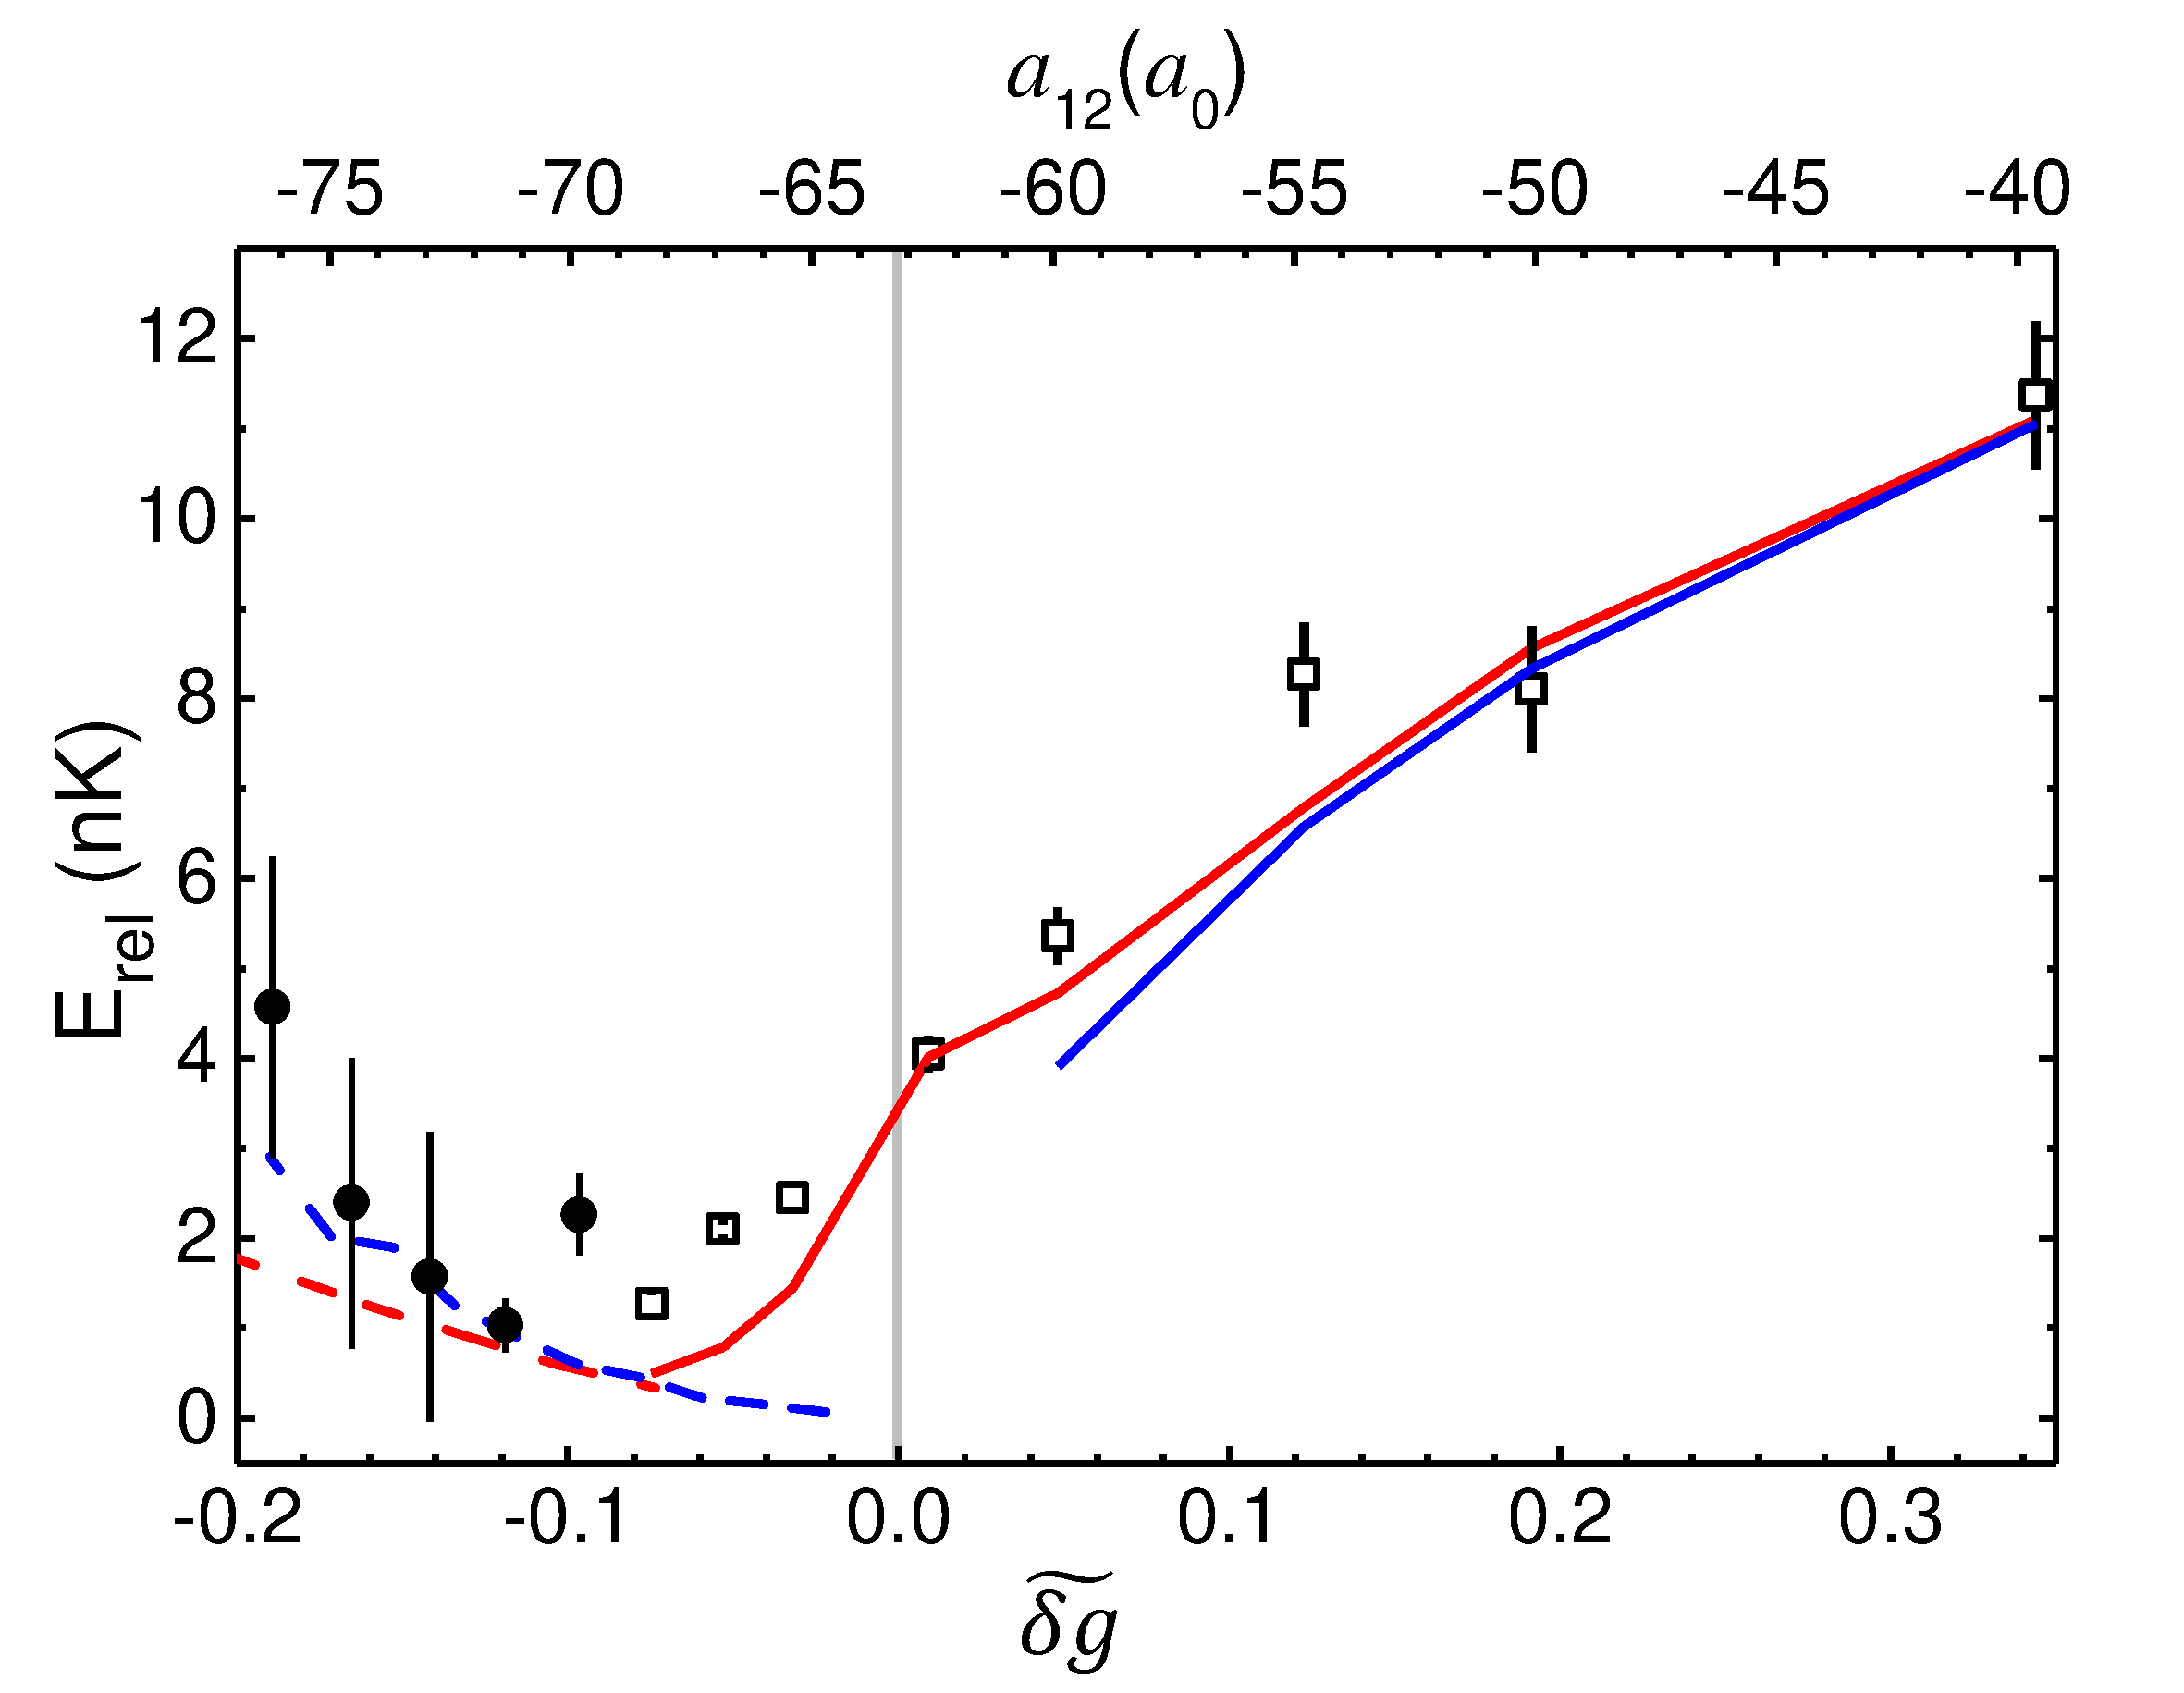
\includegraphics [width =0.85 \linewidth]{fig4.pdf}
\end{center}
\caption[Measurement of the release energy as a function of $\widetilde{\delta g}$]{Measurement of the release energy as a function of $\widetilde{\delta g}$. The open squares represent $E_{\rm rel}$ of the gas phase mixtures released from the trap directly, while the solid circles are $E_{\rm rel}$ of the gas samples formed following the liquid-gas phase transition. The red solid (blue solid) curve is the calculated $E_{\rm rel}$ with (without) the LHY terms for the first case with GPEs and the red dashed curve is $E_{\rm rel}$ for the second case from variational theory.}  
\label{fig4}
\end{figure}

We calculated the $E_{\rm rel}$ with the eGPEs for the corresponding atom numbers at the end of the TOF and found a good match for both the $E_{\rm MF}\gg E_{\rm LHY}$ and the $E_{\rm MF} \approx 0$ regions (red solid curve in Fig.~\ref{fig4}). We note that without the LHY term, the calculation fails for $\widetilde{\delta g} < 0$ due to the collapse (blue solid curve in Fig.~\ref{fig4}). At the $\widetilde{\delta g} \approx 0$ point with $E_{\rm MF}$ almost canceled, the energy difference between the two calculations is about $1$~nK. This is essentially the magnitude of $E_\text{\rm LHY}$, if we assume $E_{\rm kin}$ does not change dramatically in these two cases.   

The gas phase mixture formed following the liquid-to-gas phase transition is also of great interest. As shown in Fig.~\ref{fig2}(a), its expansion velocity can be measured and converted into another $E_{\rm rel}$ even though there is no trap involved. These results are shown in Fig.~\ref{fig4} as solid circles for $\widetilde{\delta g}$ from -0.146 to -0.247. Compared with the gas phase mixture released from the trap, the $E_{\rm rel}$ here has a completely opposite dependence on $\widetilde{\delta g}$. 

This behavior can be qualitatively understood from the change of the total energy of the droplet ($E_\text{tot}$) during the phase transition. For large enough atom numbers, $E_{\rm tot}$ has a negative minimum, and the system is in the droplet phase. Following the number loss, $E_{\rm tot}$ increases gradually. The droplet becomes meta-stable when $E_{\rm tot}$ is above zero, and the system eventually enters the gas phase when the energy minimum disappears. The measured $E_{\rm rel}$ here reflects $E_\text{tot}$ at the phase transition point which also includes contributions from $E_{\rm LHY}$, $E_{\rm MF}$, and $E_{\rm kin}$.

For more negative $\widetilde{\delta g}$, the critical atom numbers at the phase transition point are smaller, but the sample size $\propto |\widetilde{\delta g}|^{-3/2}$ shrinks much steeper. As result, the increase of the positive $E_{\rm LHY}$ and $E_{\rm kin}$ terms are faster than the decrease of the negative $E_{\rm MF}$ term. $E_{\rm tot}$ is thus positive and the measured $E_{\rm rel}$ also follows the same trend and increases for more negative $\widetilde{\delta g}$. We note that without $E_{\rm LHY}$, the magnitude of $E_{\rm MF}$ is larger than $E_{\rm kin}$ and the system will collapse. This picture is confirmed by the variational calculation as depicted by the red dashed curve in Fig.~\ref{fig4}.   

\section{Mode matching when producing droplet sample}
\label{sec:mode_match}

\subsection{In-trap vs. free-space sample}

During the release of the double BEC sample from the optical trap, the trap energy suddenly is removed suddenly but the size of the sample has no time to adapt to the new value. As shown in Fig.~\ref{figS1}, in general the in-trap size is smaller than the size of the ground-state free-space droplet at the energy minimum. The sample size will thus start to expand after released from the trap and its total energy (per particle) $E_{\rm tot} = E_{\rm kin} + E_{\rm int}$ will also start to evolve following the red curves. For the cases with very small $|\widetilde{\delta g}|$ [Fig.~\ref{figS1}(a)], $E_{\rm tot}$ is higher than the energy barrier at the right hand side. In this case, the sample will just keep expanding after crossing the maximum point and never forms the droplet. While in Fig. \ref{figS1}(b), with $|\widetilde{\delta g}|$ large enough, the negative $E_{\rm tot}$ of the released sample is not enough to overcome the energy barrier and the droplet can be formed, but its size will undergo a small-amplitude oscillation.

%% add figure-S1
\begin{figure}[hbt]
\begin{center}
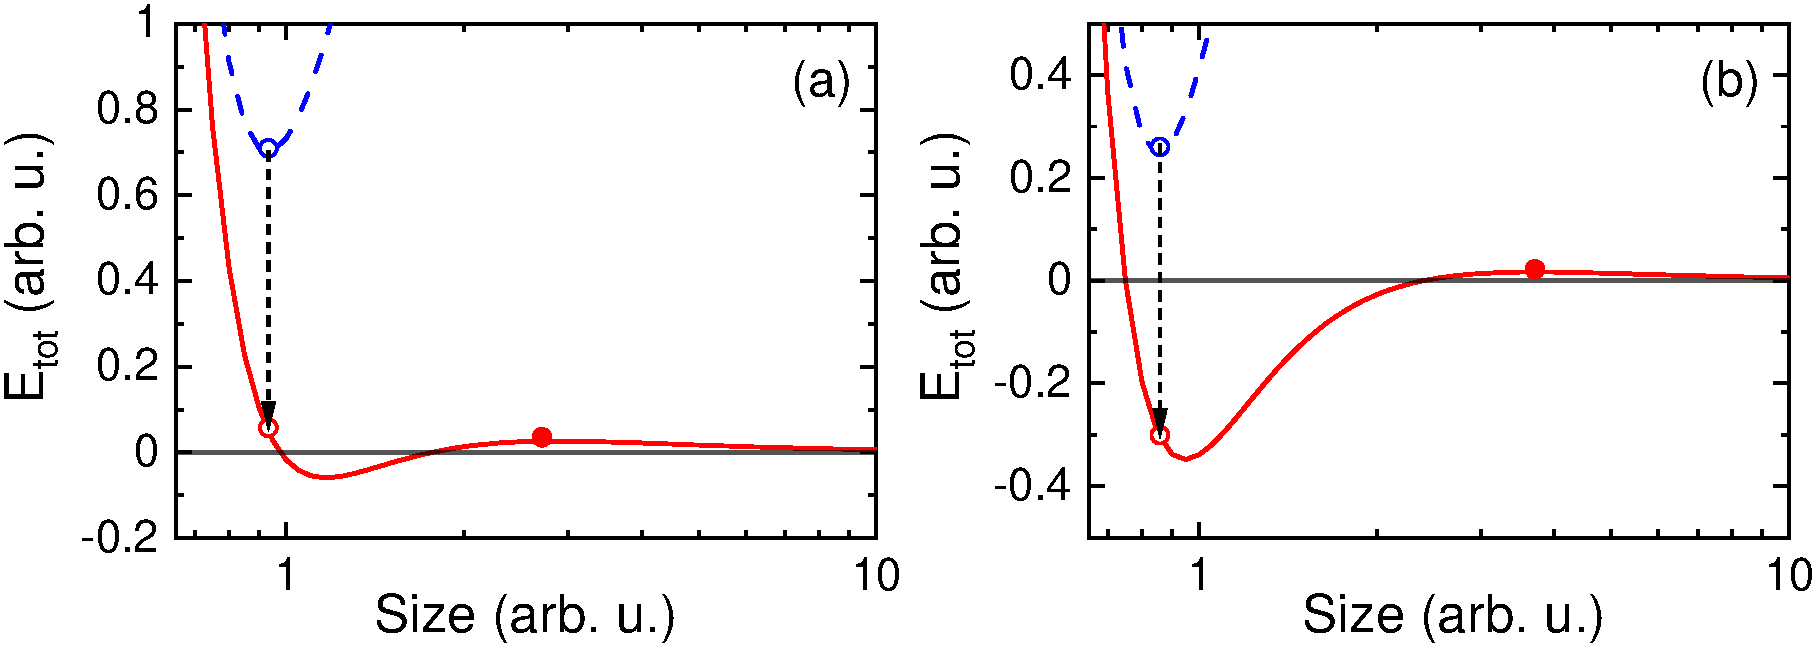
\includegraphics [width = \linewidth]{figS1.pdf}
\end{center}
\caption[Droplet formation by directly releasing the trapped sample.]{Droplet formation by directly releasing the trapped sample. The blue dashed curves represent $E_{\rm tot} = E_{\rm kin}+E_{\rm pot}+E_{\rm int}$ of the trapped double BEC, and the red solid curves are $E_{\rm tot}$ in free space (i.e., $E_{\rm kin}+E_{\rm int}$). (a) For very small $|\widetilde{\delta g}|$, the free-space $E_{\rm tot}$ (the red open circle) is higher than the barrier height on the large size side (the red solid dot). In this case, the sample will keep expanding and never forms the droplet. (b) For $|\widetilde{\delta g}|$ large enough, the sample does not have enough energy and will be confined near the energy minimum to form the droplet.}
\label{figS1}
\end{figure}

\subsection{producing weak bound droplet by quenching B-field}

To improve the mode matching, we used a nearly spherical shape trap for matching the sphere shape of the quantum droplet. In addition, as the in-trap size of the double BEC also depends strongly on $\widetilde{\delta g}$, the magnetic field is controlled in a carefully designed sequence. After the double BEC is created, the magnetic field is first ramped up quickly across the Feshbach resonance to $358.4$~G where $a_{12}$ has a small positive value of $46.1a_0$. After 350 ms for the system to stabilize, the magnetic field is ramped down to 350.451 G in 130 ms. This is just 0.424 G above $B_c$ and the corresponding $a_{12}$ is $-39.5a_0$ ($\widetilde{\delta g} = +0.322$). Here the double BEC is miscible and the attractive interaction increases the spatial overlap of the two condensates and also increases the in-trap densities substantially. Both effects significantly improve the mode matching and facilitate the free-space droplet formation. At this point, rapid atom losses are already observed; thus, the magnetic field holds here for only 10 ms. Afterwards, the magnetic field is ramped to a target value within 5 ms before the droplet is detected in free space. As depicted in Fig.~\ref{figS1}(b), although droplet can be observed after these improvements for $|\widetilde{\delta g}|$ large enough, the mode matching is not perfect. For $\widetilde{\delta g}$ from 0 to -0.146, with the current atom numbers, the droplet cannot be observed by simply releasing the double BEC from the trap. As shown in Fig.~\ref{figS2}(a), even better mode matching can be achieved by finding a $\widetilde{\delta g}$ value where the in-trap size matches with the target droplet size and quenches $\widetilde{\delta g}$ at the same time when the trap is shut off. To achieve the fast magnetic field quenching necessary for this method, we added a small magnetic coil which is capable of covering the magnetic field range in less than 10 $\mu$s. Fig.~\ref{figS2}(b) and (c) show two droplets formed with this method. For case (b) with $\widetilde{\delta g} = -0.141$, the droplet lifetime is longer than the available observation time. For case (c) with $\widetilde{\delta g} = -0.110$, the liquid-to-gas phase transition is observed after about 7 ms. This short lifetime is probably limited by the atom numbers since at this $\widetilde{\delta g}$, the critical atom numbers are much larger.

\begin{figure}[hbtp]
\begin{center}
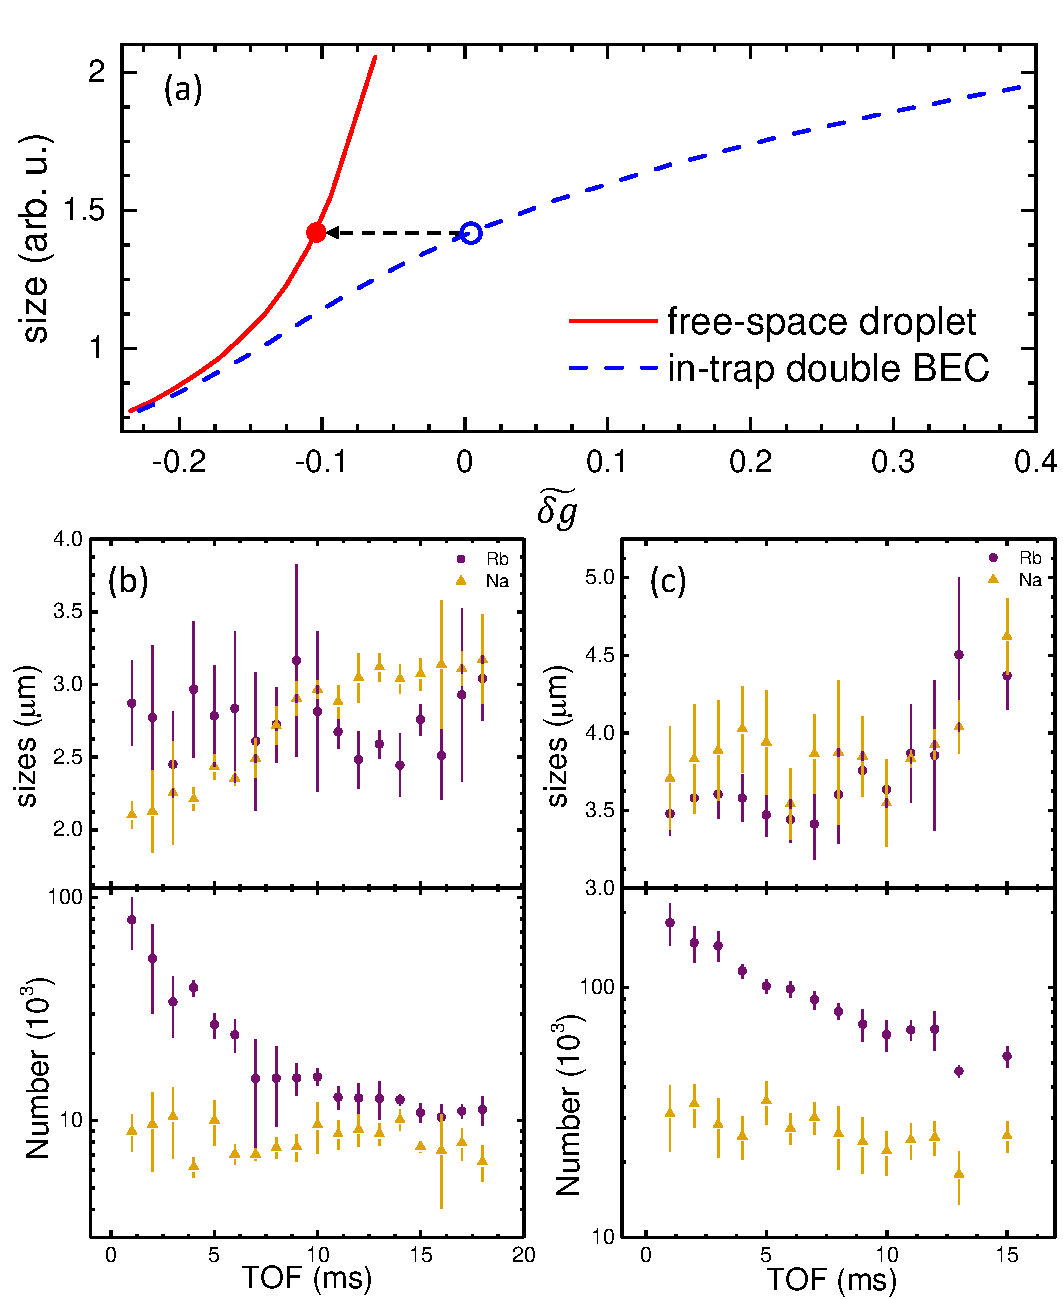
\includegraphics [width = 0.85 \linewidth]{figS2.pdf}
\end{center}
\caption[Producing long-lived droplet by magnetic field quench]{Producing long-lived droplet by magnetic field quench. (a) For some weakly bound droplet, it is possible to find a $\widetilde{\delta g}$ 
value where the in-trap gas-phase sample size (blue dashed curve) is the same as the size of the free-space droplet (red solid curve). Quenching $\widetilde{\delta g}$ at the instant of releasing the sample, as depicted by the black dashed arrow, will lead to a near perfect mode matching. (b) and (c) show the experimentally measured droplet signals for $\widetilde{\delta g} = -0.141$ (349.880 G) and $\widetilde{\delta g} = -0.110$ (349.910 G) created with this method. At these magnetic fields, no 
droplet can be observed without the quench as they fall in the situation as described in Fig.~\ref{figS1}(a).}
\label{figS2}
\end{figure}

\section{producing Feshbach molecule from droplet}
\label{sec:droplet_molecule}